%Version 3 October 2023
% See section 11 of the User Manual for version history
%
%%%%%%%%%%%%%%%%%%%%%%%%%%%%%%%%%%%%%%%%%%%%%%%%%%%%%%%%%%%%%%%%%%%%%%
%%                                                                 %%
%% Please do not use \input{...} to include other tex files.       %%
%% Submit your LaTeX manuscript as one .tex document.              %%
%%                                                                 %%
%% All additional figures and files should be attached             %%
%% separately and not embedded in the \TeX\ document itself.       %%
%%                                                                 %%
%%%%%%%%%%%%%%%%%%%%%%%%%%%%%%%%%%%%%%%%%%%%%%%%%%%%%%%%%%%%%%%%%%%%%

%%\documentclass[referee,sn-basic]{sn-jnl}% referee option is meant for double line spacing

%%=======================================================%%
%% to print line numbers in the margin use lineno option %%
%%=======================================================%%

%%\documentclass[lineno,sn-basic]{sn-jnl}% Basic Springer Nature Reference Style/Chemistry Reference Style

%%======================================================%%
%% to compile with pdflatex/xelatex use pdflatex option %%
%%======================================================%%

%%\documentclass[pdflatex,sn-basic]{sn-jnl}% Basic Springer Nature Reference Style/Chemistry Reference Style


%%Note: the following reference styles support Namedate and Numbered referencing. By default the style follows the most common style. To switch between the options you can add or remove `Numbered` in the optional parenthesis. 
%%The option is available for: sn-basic.bst, sn-vancouver.bst, sn-chicago.bst%  
 
%%\documentclass[sn-nature]{sn-jnl}% Style for submissions to Nature Portfolio journals
%%\documentclass[sn-basic]{sn-jnl}% Basic Springer Nature Reference Style/Chemistry Reference Style
\documentclass[sn-mathphys-num]{sn-jnl}% Math and Physical Sciences Numbered Reference Style 
%%\documentclass[sn-mathphys-ay]{sn-jnl}% Math and Physical Sciences Author Year Reference Style
%%\documentclass[sn-aps]{sn-jnl}% American Physical Society (APS) Reference Style
%%\documentclass[sn-vancouver,Numbered]{sn-jnl}% Vancouver Reference Style
%%\documentclass[sn-apa]{sn-jnl}% APA Reference Style 
%%\documentclass[sn-chicago]{sn-jnl}% Chicago-based Humanities Reference Style

\graphicspath{{figs}}

%%%% Standard Packages
%%<additional latex packages if required can be included here>

\usepackage{graphicx}%
\usepackage{multirow}%
\usepackage{amsmath,amssymb,amsfonts}%
\usepackage{amsthm}%
\usepackage{mathrsfs}%
\usepackage[title]{appendix}%
\usepackage{xcolor}%
\usepackage{textcomp}%
\usepackage{manyfoot}%
\usepackage{booktabs}%
\usepackage{algorithm}%
\usepackage{algorithmicx}%
\usepackage{algpseudocode}%
\usepackage{listings}%
%%%%

\newcommand{\myfigref}[2]{~\ref{#1}.\subref{#2}}% <---- a new macro for referring to a subfigure
\usepackage{subfig} % for subfigures
\usepackage{wrapfig}

%%%%%=============================================================================%%%%
%%%%  Remarks: This template is provided to aid authors with the preparation
%%%%  of original research articles intended for submission to journals published 
%%%%  by Springer Nature. The guidance has been prepared in partnership with 
%%%%  production teams to conform to Springer Nature technical requirements. 
%%%%  Editorial and presentation requirements differ among journal portfolios and 
%%%%  research disciplines. You may find sections in this template are irrelevant 
%%%%  to your work and are empowered to omit any such section if allowed by the 
%%%%  journal you intend to submit to. The submission guidelines and policies 
%%%%  of the journal take precedence. A detailed User Manual is available in the 
%%%%  template package for technical guidance.
%%%%%=============================================================================%%%%

%% as per the requirement new theorem styles can be included as shown below
\theoremstyle{thmstyleone}%
\newtheorem{theorem}{Theorem}%  meant for continuous numbers
%%\newtheorem{theorem}{Theorem}[section]% meant for sectionwise numbers
%% optional argument [theorem] produces theorem numbering sequence instead of independent numbers for Proposition
\newtheorem{proposition}[theorem]{Proposition}% 
%%\newtheorem{proposition}{Proposition}% to get separate numbers for theorem and proposition etc.

\theoremstyle{thmstyletwo}%
\newtheorem{example}{Example}%
\newtheorem{remark}{Remark}%

\theoremstyle{thmstylethree}%
\newtheorem{definition}{Definition}%

\raggedbottom
%%\unnumbered% uncomment this for unnumbered level heads

% transpose
\newcommand{\T}{^{\mathsf{T}}}

\begin{document}

\title{Forecasting fMRI Images From Video Sequences: Linear Model Analysis}

%%=============================================================%%
%% GivenName	-> \fnm{Joergen W.}
%% Particle	-> \spfx{van der} -> surname prefix
%% FamilyName	-> \sur{Ploeg}
%% Suffix	-> \sfx{IV}
%% \author*[1,2]{\fnm{Joergen W.} \spfx{van der} \sur{Ploeg} 
%%  \sfx{IV}}\email{iauthor@gmail.com}
%%=============================================================%%

\author*[1]{\fnm{Daniil} \sur{Dorin}}\email{dorin.dd@phystech.edu}
\equalcont{These authors contributed equally to this work.}

\author[1]{\fnm{Nikita} \sur{Kiselev}}\email{kiselev.ns@phystech.edu}
\equalcont{These authors contributed equally to this work.}

\author[1]{\fnm{Andrey} \sur{Grabovoy}}\email{grabovoy.av@phystech.edu}

\affil[1]{\orgdiv{Department of Intelligent Systems}, \orgname{Moscow Institute of Physics and Technology}, \orgaddress{\street{9 Institutskiy per.}, \city{Dolgoprudny}, \postcode{141701}, \state{Moscow Region}, \country{Russia}}}

%%==================================%%
%% Sample for unstructured abstract %%
%%==================================%%

\abstract{The issue of reconstructing the relationship between functional magnetic resonance imaging (fMRI) sensor readings and human perception of the external is investigated. The study analyzes the dependence between the fMRI images and the videos viewed by individuals. Based on this analysis, a method is proposed for approximating the fMRI readings using the video sequence. The method is based on the assumption that there is a time-invariant hemodynamic response to changes in blood oxygen levels. A linear model is constructed for each individual voxel in the fMRI image, assuming that the image sequence follows a Markov property. To test the proposed method, a computational experiment was conducted on a dataset collected during tomographic examinations of a large number of individuals. The performance of the method was evaluated based on the experimental data, and hypotheses were tested regarding the invariance of the model weights and the correctness of the method.}

\keywords{neuroimaging, fMRI, video sequences, correlation analysis, hypothesis testing, linear model, forecasting}

%%\pacs[JEL Classification]{D8, H51}

%%\pacs[MSC Classification]{35A01, 65L10, 65L12, 65L20, 65L70}

\maketitle

\section{Introduction}

A set of techniques used to visualize the structure and function of the human brain is called \textit{neurovisualization}. Neuroimaging \cite{puras2014neurovisualization} techniques, such as electrocardiography (ECG), computed tomography (CT), magnetic resonance imaging (MRI), and functional magnetic resonance imaging (fMRI), are used to study the brain and detect diseases and mental disorders.

\textit{Functional magnetic resonance imaging}, or \textit{fMRI}, is a type of magnetic resonance imaging  that measures changes in blood flow in the brain. These changes are caused by neural activity \cite{Glover2011} and occur with a delay of 4--8 seconds \cite{Bandettini1992}, due to the time it takes for the vascular system to respond to the brain's demand for glucose \cite{Ogawa1990, LEBIHAN1995231, Logothetis2003}. This delayed response is essential for accurate fMRI measurements, as it allows for the detection of neural activity that occurs over a longer period of time.

In fMRI imaging, sequences of echo-planar imaging (EPI) are used \cite{Connelly1993, Kwong1992, Ogawa1992}. The processing of areas with varying signal intensities, depending on the method of activation and the type of artifact, is carried out using specialized methods and software \cite{Bandettini1992, BAUDENDISTEL1995701, COX1996162}. The processed results are then formalized as activation maps, which can be combined with the localization of anatomical structures in the cerebral cortex.

The fMRI technique plays a significant role in neuroimaging, although it has some significant limitations. The works of \cite{menon1999spatial} and \cite{logothetis2008we} discuss the temporal and spatial resolution of fMRI, with the latter emphasizing the significant disadvantage of temporal resolution. Another limitation of fMRI is the inevitable noise associated with movement, such as that caused by the heartbeat and respiration of the subject, as well as thermal fluctuations of the scanner itself. In the paper \cite{1804.10167}, graph-based techniques are proposed to address these issues and demonstrate their effectiveness in tasks such as epilepsy and depression detection. These methods aim to suppress the noise mentioned above and improve the accuracy of the results.

In fMRI, the participant is given a variety of tasks and external stimuli, which induce activation of specific areas of the brain. These stimuli include movements of fingers and limbs \cite{Roux1998, Papke1999}, image finding and examination of a chessboard \cite{Engel1994, Schneider1994}, listening to non-specific noises, and reading single words or coherent text \cite{Binder1994, Dymarkowski1998}. Changes in brain activity during the fMRI examination could also be caused by watching a video  \cite{decety1997brain}, which is the focus of this study.

The most well-known video processing techniques are based on 3D convolutional neural networks \cite{tran2015learning}. The main difference between 3D and 2D convolution is that the former processes the spatial and temporal information simultaneously. However, this approach has some drawbacks, such as an increase in the number of parameters and computational complexity. One of the most advanced and promising architectures for image processing is ResNet \cite{he2015deep}. This network allows training deep neural networks with up to 152 layers, overcoming the issue of gradient vanishing that occurs during training of deep networks. ResNet achieves high accuracy and has become a standard for image classification and object detection tasks.

The main focus of the research is to investigate the relationship between fMRI images and video recordings. It is assumed that such a relationship exists, and it is hypothesized that there may be a consistent time lag between fMRI images and corresponding video frames \cite{Logothetis2003}. The study investigates the relationship between an individual fMRI image and the preceding image. The time delay between these images serves as a hyperparameter in the model, which is used to approximate fMRI images based on a given video sequence.

According to a study \cite{anderson2006}, when patients undergo fMRI, viewing a video activates a specific network of brain regions. This network, which includes the occipital lobe and frontal regions, is located predominantly in the right hemisphere. In this paper, we are considering an approach that utilizes these brain regions to analyze latency times.

The data on which the dependency hypothesis is tested and the demonstration of the work of the constructed method are presented in paper \cite{Berezutskaya2022}. This dataset was obtained by examining a group of 63 subjects, thirty of whom underwent fMRI scanning. They were asked to complete the same task, which was to watch a short audio visual film. Annotations were generated for this task in the paper under review, including information about the timing of the appearance and disappearance of individual words, objects, and characters. Detailed descriptions of the methods for audio and video annotation can be found in \cite{boersma2018praat} and \cite{Berezutskaya2020}.

\section{Problem statement}

Frame rate $\nu \in \mathbb{R}$ and duration $t \in \mathbb{R}$ of the video sequence are set. The video sequence is set as
\begin{equation*}
	\label{eq1}
	\mathbf{P} = [\mathbf{p}_1, \ldots, \mathbf{p}_{\nu t}], \quad\
	\mathbf{p}_{\ell} \in \mathbb{R}^{W \times H \times C},
\end{equation*}
with width, height and number of image channels $W, H$ and $C$, respectively.

Let us denote the frequency of fMRI images by $\mu \in \mathbb{R}$. We set the sequence of images
\begin{equation*}
	\label{eq2}
	\mathbf{S} = [\mathbf{s}_1, \ldots, \mathbf{s}_{\mu t}], \quad\
	\mathbf{s}_{\ell} \in \mathbb{R}^{X \times Y \times Z},
\end{equation*}
where $X, Y$, and $Z$~--- the dimensions of the voxel image.

The problem is to construct a mapping that accounts for the $\Delta t$ delay between the fMRI image and the video sequence, as well as previous tomographic readings. fMRI image and the video sequence, as well as previous tomographic readings. Formally, it is necessary to find such a mapping $\mathbf{g}$ that
\begin{equation*}
	\label{eq3}
	\mathbf{g}(\mathbf{p}_1, \ldots, \mathbf{p}_{k_{\ell} - \nu \Delta t}; \mathbf{s}_1, \ldots, \mathbf{s}_{\ell-1}) = \mathbf{s}_{\ell}, \quad \ell = 1, \ldots, \mu t,
\end{equation*}
where for the $\ell$-th fMRI image the number of the corresponding image $k_{\ell}$ is determined by the formula
\begin{equation*}
	\label{eq4}
	k_{\ell} = \dfrac{\ell \cdot \nu}{\mu}.
\end{equation*}

\section{Proposed forecasting method}

The scheme of the proposed fMRI image reconstruction method is shown in Figure~\ref{fig:scheme}. 

\begin{figure}[h!]
	\centering
	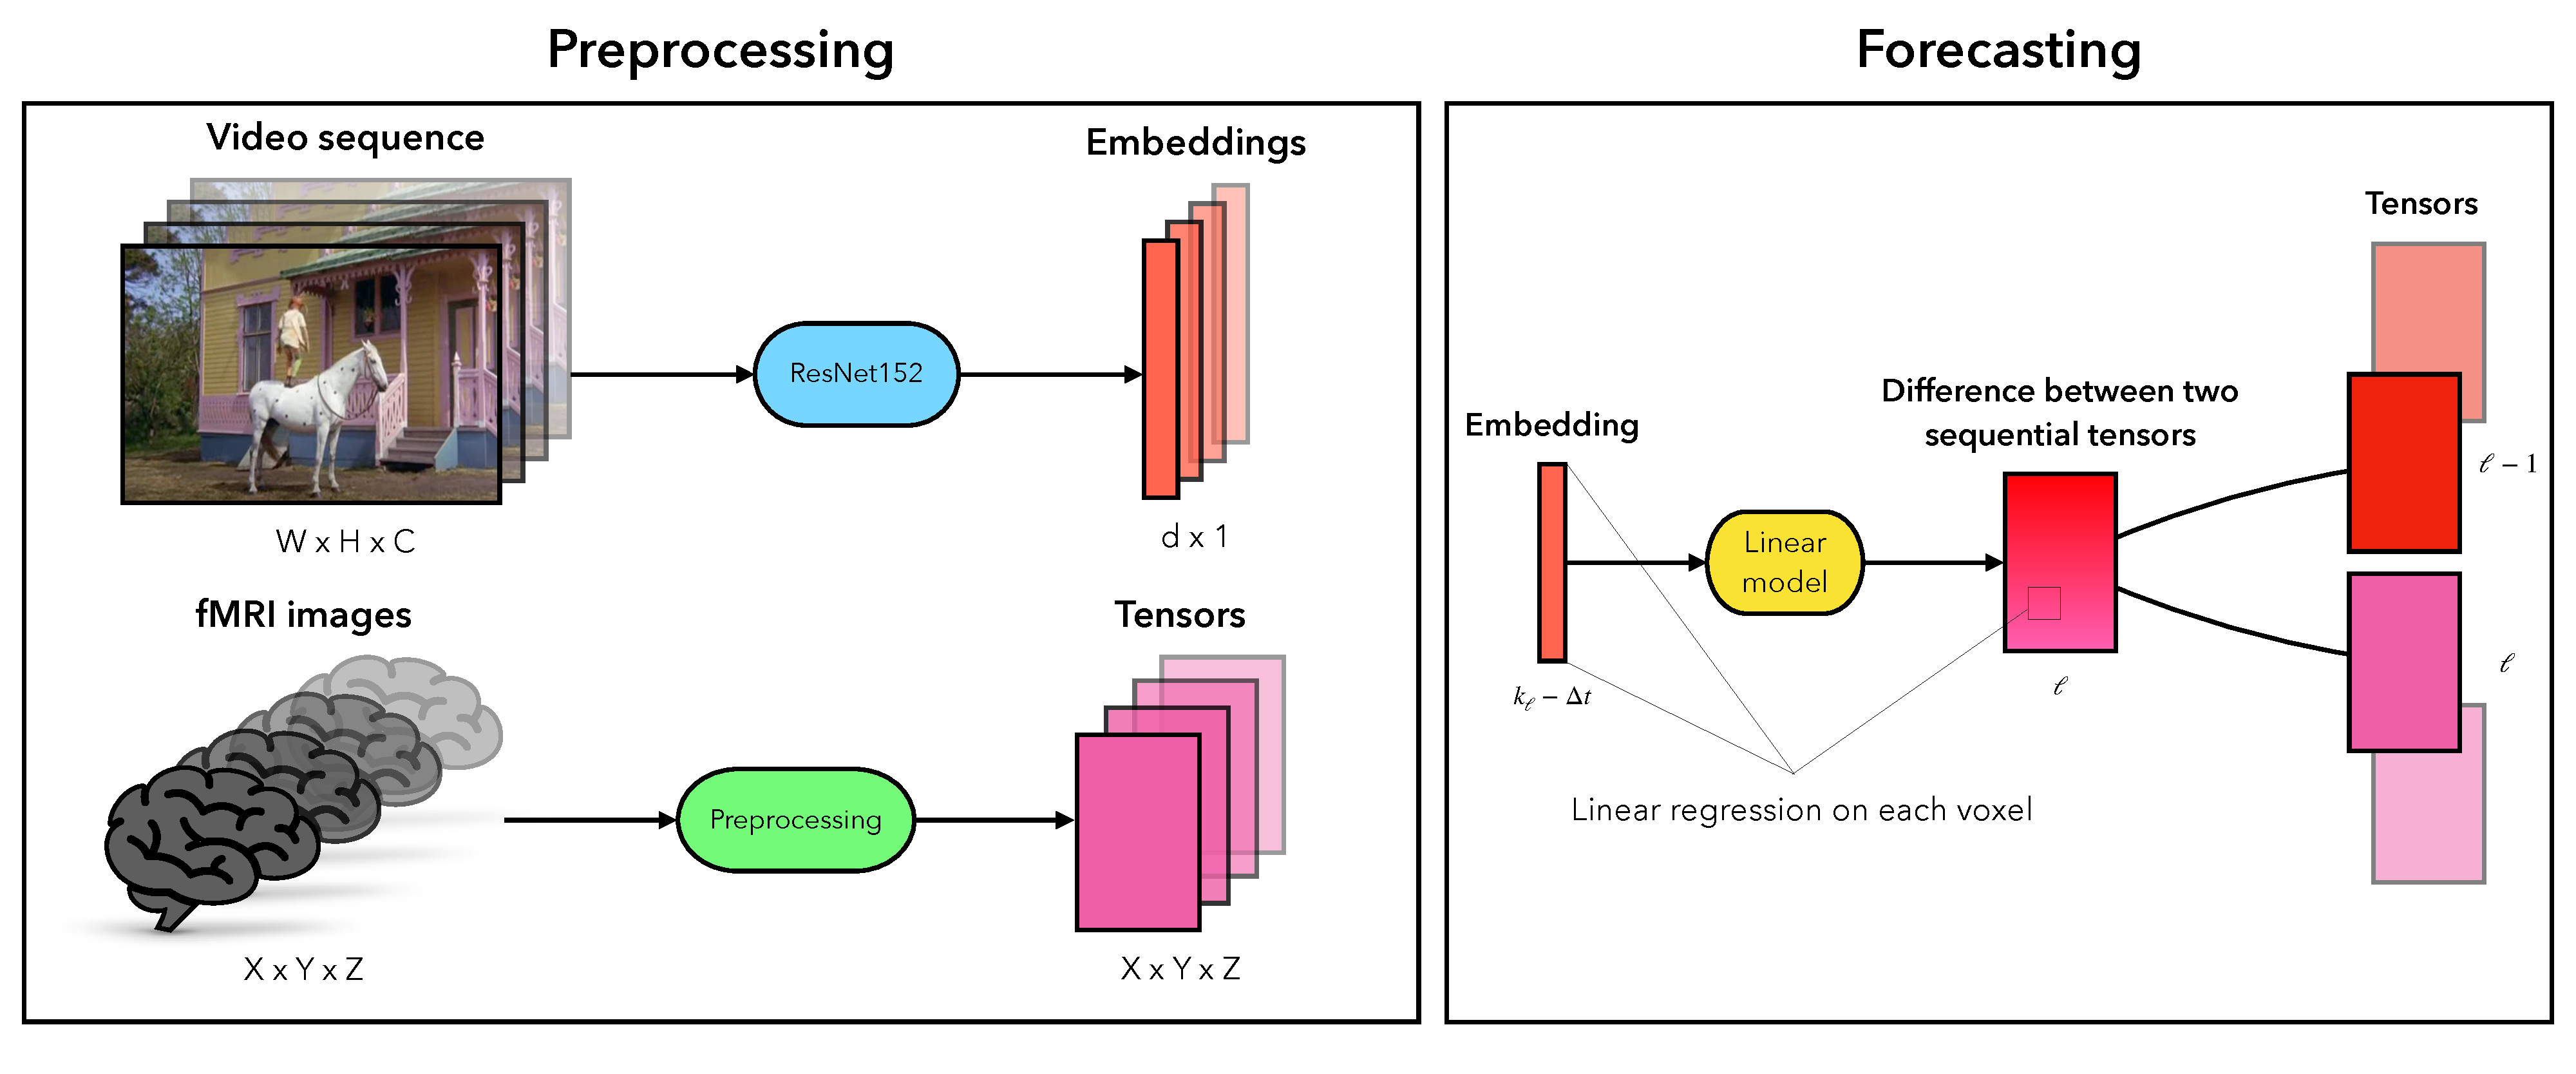
\includegraphics[width=\textwidth]{scheme.pdf}
	\caption{Method scheme}
	\label{fig:scheme}
\end{figure}

We denote the fMRI image as $\mathbf{s}_{\ell} = [v^{\ell}_{ijk}] \in \mathbb{R}^{X \times Y \times Z}$, where $v^{\ell}_{ijk} \in \mathbb{R}_+$~--- value of the corresponding voxel. In order to reduce the running time of the method, we propose to use compression of fMRI images by dimensionality reduction. Compression by a factor of 2 is represented in the form of a mapping
\[\boldsymbol{\chi}: \mathbb{R}^{X \times Y \times Z} \to \mathbb{R}^{X/2 \times Y/2 \times Z/2}.\]
A compression of $2^k$ times is obtained by applying $\boldsymbol{\chi}$ successively $k$ times.  In the following, for simplicity, we keep the notation of image dimensions $X \times Y \times Z$.

Suppose that the Markov property is satisfied for the sequence of snapshots, i.e., each snapshot depends only on one image and the previous snapshot. Then the corresponding mapping is written in the form
\begin{equation*}
	\label{eq5}
	\mathbf{g}(\mathbf{p}_{k_{\ell} - \nu \Delta t}) = \mathbf{s}_{\ell} - \mathbf{s}_{\ell-1} = \boldsymbol{\delta}_{\ell}, \quad \ell = 2, \ldots, \mu t.
\end{equation*}
where $\boldsymbol{\delta}_{\ell} = [v^{\ell}_{ijk} - v^{\ell-1}_{ijk}] = [\delta^{\ell}_{ijk}] \in \mathbb{R}^{X \times Y \times Z}$~--- the difference between two consecutive snapshots.

Mapping $\mathbf{g}: \mathbf{P} \to \mathbf{S}$ is represented as a composition of the other two:
\[ \mathbf{g} = \boldsymbol{\varphi} \circ \boldsymbol{\psi}, \]
where
\begin{align*}
	 & \boldsymbol{\psi}: \mathbf{P} \to \mathbb{R}^d
	\text{~--- image vectorization,}        \\
	 & \boldsymbol{\varphi}: \mathbb{R}^d \to \mathbf{S}
	\text{~--- target mapping.}
\end{align*}

For each image from the video sequence, we have an embedding vector of dimension $d$:
\[ \mathbf{x}_{\ell} = [x^{\ell}_1, \ldots, x^{\ell}_{d}]\T \in \mathbb{R}^{d}, \quad {\ell} = 1, \ldots, \nu t. \]
The ResNet152 neural network architecture without the last linear layer is used.

Given $k_{\ell} = \ell \cdot \nu / \mu$, the total number of pairs (image, snapshot) is $N = \mu (t - \Delta t)$. Thus, for each voxel a sample is given
\[ \mathfrak{D}_{ijk} = \{(\mathbf{x}_{\ell}, \delta^{\ell}_{ijk}) \ | \ {\ell} = 2, \ldots, N \}. \]

The regression task is set
\begin{equation*}
	\label{eq6}
	y_{ijk}: \mathbb{R}^{d} \to \mathbb{R}.
\end{equation*}

A linear model is used with a vector of parameters
\[ \mathbf{w}_{ijk} = [w^{ijk}_1, \ldots, w^{ijk}_{d}]\T \in \mathbb{R}^{d}: \]
\begin{equation*}
	\label{eq7}
	f_{ijk}(\mathbf{x}, \mathbf{w}_{ijk}) = \langle \mathbf{x}, \mathbf{w}_{ijk} \rangle.
\end{equation*}

For the model $f_{ijk}$ with its corresponding parameter vector $\mathbf{w}_{ijk} \in \mathbb{R}^{d}$ define a quadratic loss function with $L_2$ regularization:
\begin{equation*}
	\label{eq8}
	\mathcal{L}_{ijk}(\mathbf{w}_{ijk}) = \sum\limits_{\ell = 2}^{N} \big(f_{ijk}(\mathbf{x}_{\ell}, \mathbf{w}_{ijk}) - \delta^{\ell}_{ijk}\big)^2 + \alpha \| \mathbf{w}_{ijk} \|_2^2,
\end{equation*}
where $\alpha \in \mathbb{R}$~--- regularization coefficient.

It is required to find the parameters that give a minimum to the loss functional $\mathcal{L}_{ijk}(\mathbf{w}_{ijk})$ for given hyperparameters $\Delta t$ and $\alpha$:
\begin{equation*}
	\label{eq9}
	\hat{\mathbf{w}}_{ijk} = \arg\min_{\mathbf{w}_{ijk}} \mathcal{L}_{ijk}(\mathbf{w}_{ijk}).
\end{equation*}

The minimum of the loss function is found by the least squares method. Let's define the matrix of objects-features
\begin{equation*}
	\label{eq10}
	\mathbf{X} = [\mathbf{x}_2, \ldots, \mathbf{x}_N]\T = [x^i_j] \in \mathbb{R}^{(N-1) \times d}
\end{equation*}
and a vector whose components are the differences of values of the same voxel in different images,
\begin{equation*}
	\label{eq11}
	\mathbf{\Delta}_{ijk} = [\delta^2_{ijk}, \ldots, \delta^N_{ijk}]\T \in \mathbb{R}^{N-1}.
\end{equation*}

The solution is written in the form
\begin{equation*}
	\label{eq12}
	\hat{\mathbf{w}}_{ijk} = (\mathbf{X}\T \mathbf{X} + \alpha \mathbf{I})^{-1} \mathbf{X}\T \mathbf{\Delta}_{ijk}.
\end{equation*}

Let us obtain a formula for reconstructed fMRI images. Let's introduce a matrix of weights
\begin{equation*}
	\label{eq13}
	\hat{\mathbf{W}} = [\hat{\mathbf{w}}_1, \ldots, \hat{\mathbf{w}}_{XYZ}]\T = [\hat{w}^i_j] \in \mathbb{R}^{XYZ \times d}.
\end{equation*}

Let's introduce for tensors $\mathbf{s}_{\ell}, \boldsymbol{\delta}_{\ell} \in \mathbb{R}^{X \times Y \times Z}$ vectors
\[ \mathbf{s}_{\ell}^{R} = [ v^{\ell}_1, \ldots, v^{\ell}_{XYZ} ]\T,\
	\boldsymbol{\delta}_{\ell}^{R} = [ \delta^{\ell}_1, \ldots, \delta^{\ell}_{XYZ} ]\T \in \mathbb{R}^{XYZ}. \]

Then the vector of the forecasted image is found by the formula
\begin{equation*}
	\label{eq14}
	\hat{\mathbf{s}}_{\ell}^{R} = \mathbf{s}_{\ell-1}^{R} + \hat{\boldsymbol{\delta}}_{\ell}^{R} = \mathbf{s}_{\ell-1}^{R} + \hat{\mathbf{W}} \mathbf{x}_{\ell}.
\end{equation*}

\section{Numerical experiment}

To analyze the performance of the proposed method and test the hypotheses a computational experiment was carried out.

The sample presented in \cite{Berezutskaya2022} was used as data.
The dataset contains the results of examination of 63 subjects.
For thirty of them fMRI readings are known.
There are 16 males and 14 females, ranging in age from 7 to 47 years.
The mean age of the subjects~--- 22 years.

Characteristics of the sample: duration of examination,
frame rates of fMRI video sequences and images, and their dimensions are summarized in Table~\ref{table:sample}.

\begin{table}[h!]
\caption{Dataset Description}\label{table:sample}
\begin{tabular}{@{}ccc@{}}
\toprule
Name & Notation & Value \\ 
\midrule
Duration of examination & $t$ & 390 s \\
Video frame rate & $\nu$ & 25 Hz \\
fMRI frame rate & $\mu$ & 1.64 Hz \\
Video dimensions & $W, H, C$ & 640, 480, 3 \\
fMRI dimensions & $X, Y, Z$ & 40, 64, 64 \\
\botrule
\end{tabular}
\end{table}

The sample was divided into training and test samples in the ratio of 70\% and 30\%, respectively.
The quality criterion for fMRI image reconstruction is MSE~--- the sum of squares of deviations
between the true and reconstructed images, averaged over all voxels of each image.
from the test sample.

To reduce the running time of the algorithm, the fMRI image is precompressed
using MaxPool3D layer. Compression ratios of 1, 2, 4 and 8 are considered.
The voxel values are normalized to $[0; 1]$ by the MinMaxScale procedure.

Table~\ref{table:pc} summarizes the specifications of the computer on which the computational experiment was
on which the computational experiment was performed.

\begin{table}[h!]
\caption{PC Specification}\label{table:pc}
\begin{tabular}{@{}cc@{}}
\toprule
Element & Description \\
\midrule
CPU & Intel Core i7-7700 3.6 GHz \\
GPU & NVIDIA GeForce GTX 1060 3 GB \\
RAM & 16 GB 2400 MHz \\
Hard Drive & M.2 SSD \\
OS & Windows 10 \\
\botrule
\end{tabular}
\end{table}

\subsection{Method performance}

Figure~\ref*{fig:example} shows slices of the true and reconstructed images from the test sample.
Figure\myfigref{fig:example}{fig:example-c} shows the difference between them.
To demonstrate the performance of the algorithm, the 7th subject was selected, $\Delta t = 5 \text{s}$, compression factor 1, regularization factor
$\alpha = 1000$. The 20th slice along the first coordinate of the 37th image in the sequence was considered.
Since the voxel values are normalized to the segment $[0; 1]$, an error of the order of $10^{-3}$
indicates a fairly accurate prediction.

\begin{figure}[h!]
	\centering
	\subfloat[Test]{\label{fig:example-a}{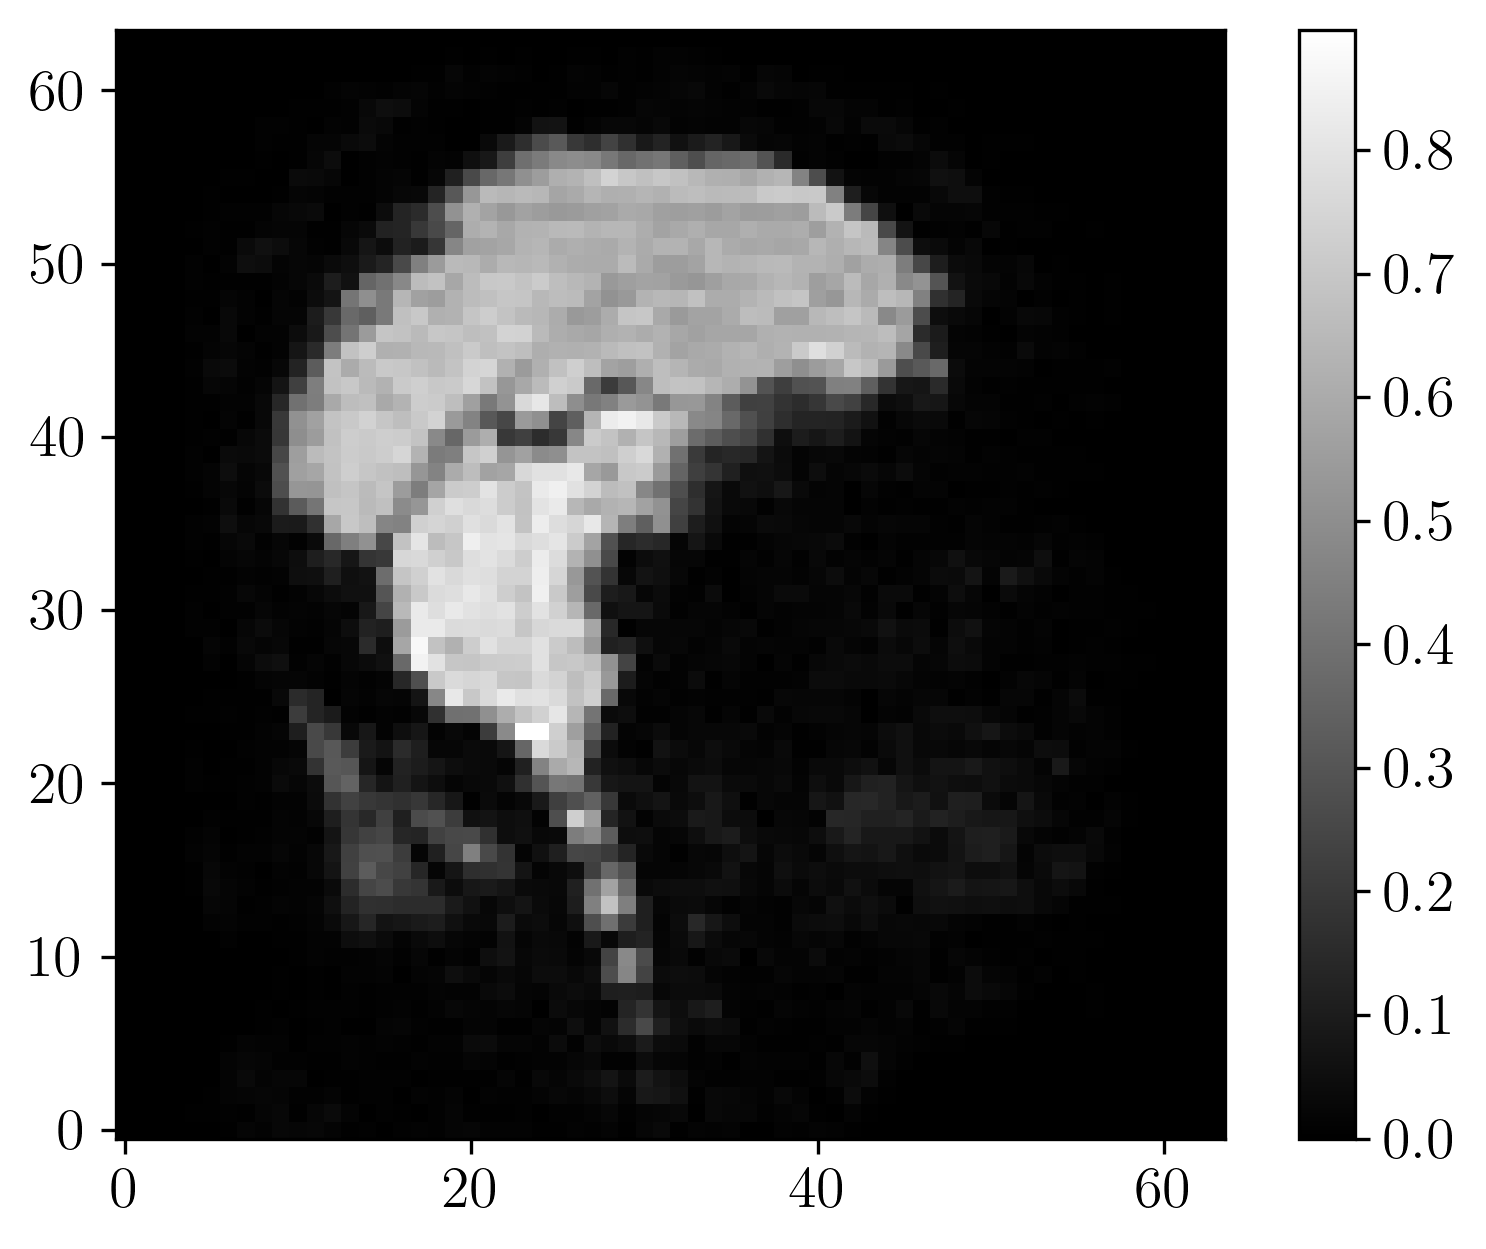
\includegraphics[width=0.33\textwidth]{default/sub-07-5-1-1000-37-20-_-_-test.png}}}
	\hfill
	\subfloat[Predicted]{\label{fig:example-b}{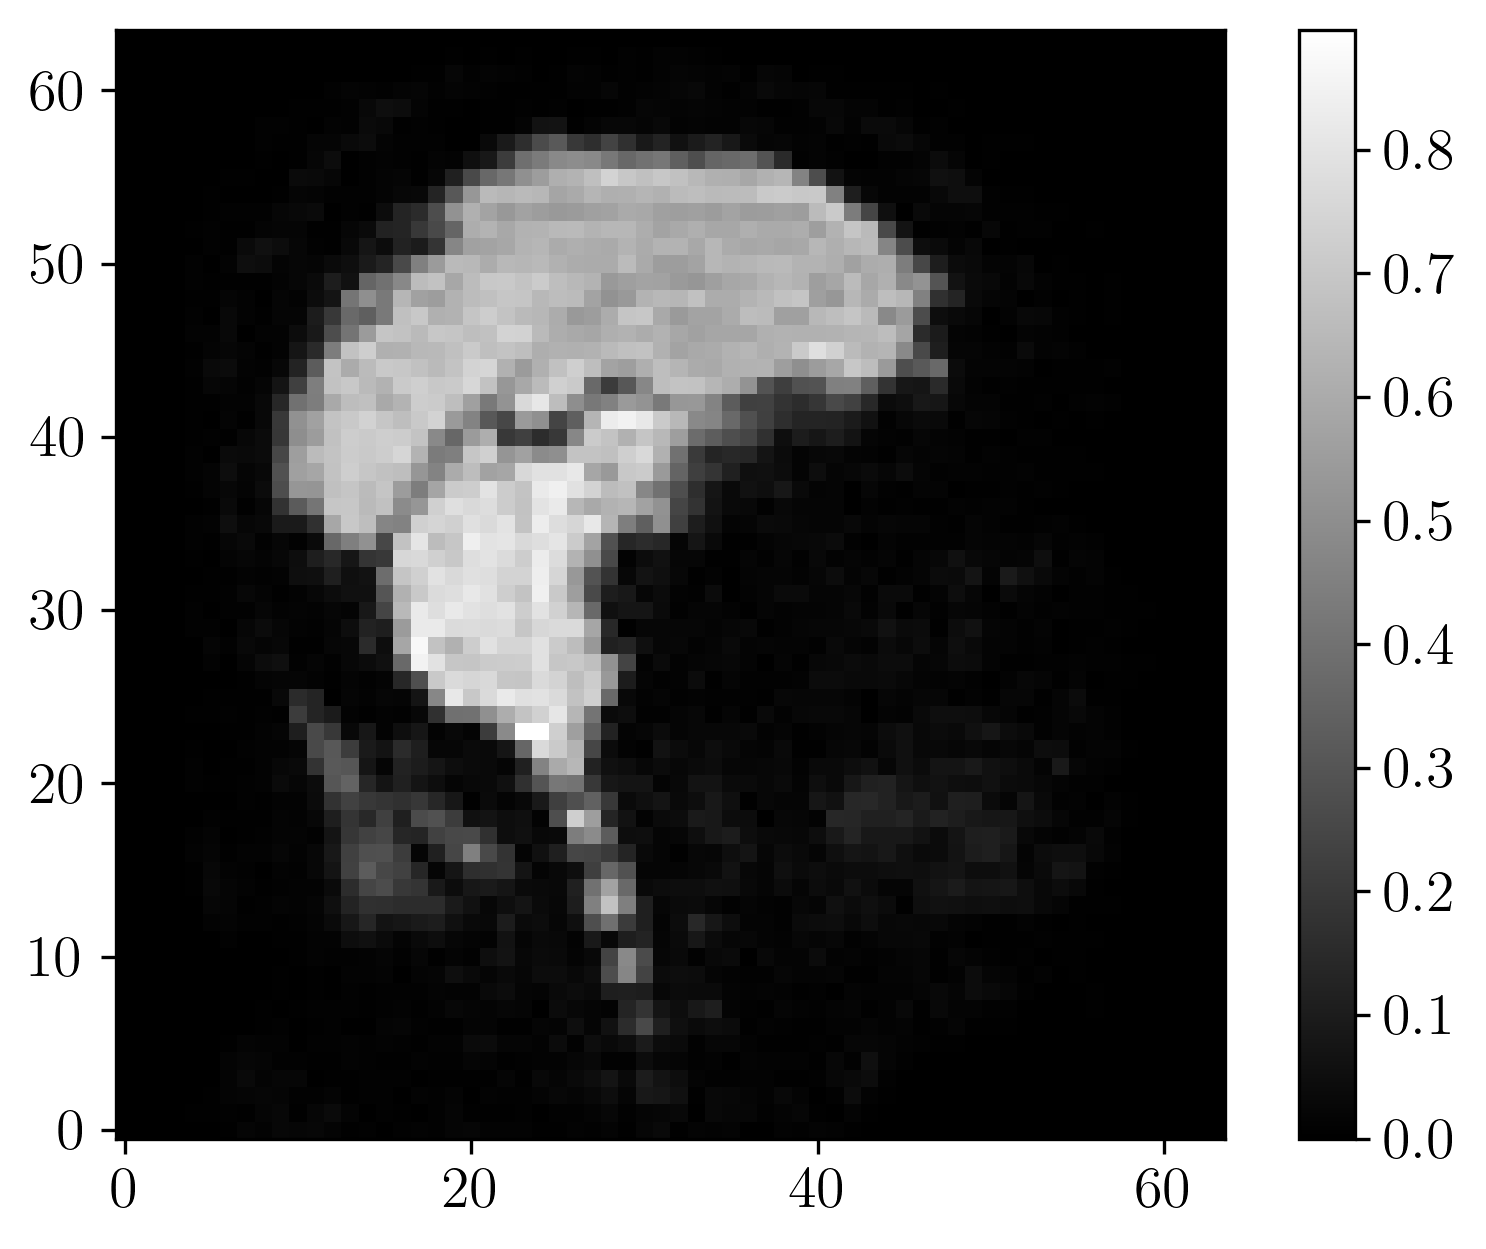
\includegraphics[width=0.33\textwidth]{default/sub-07-5-1-1000-37-20-_-_-predicted.png}}}
	\hfill
	\subfloat[Difference]{\label{fig:example-c}{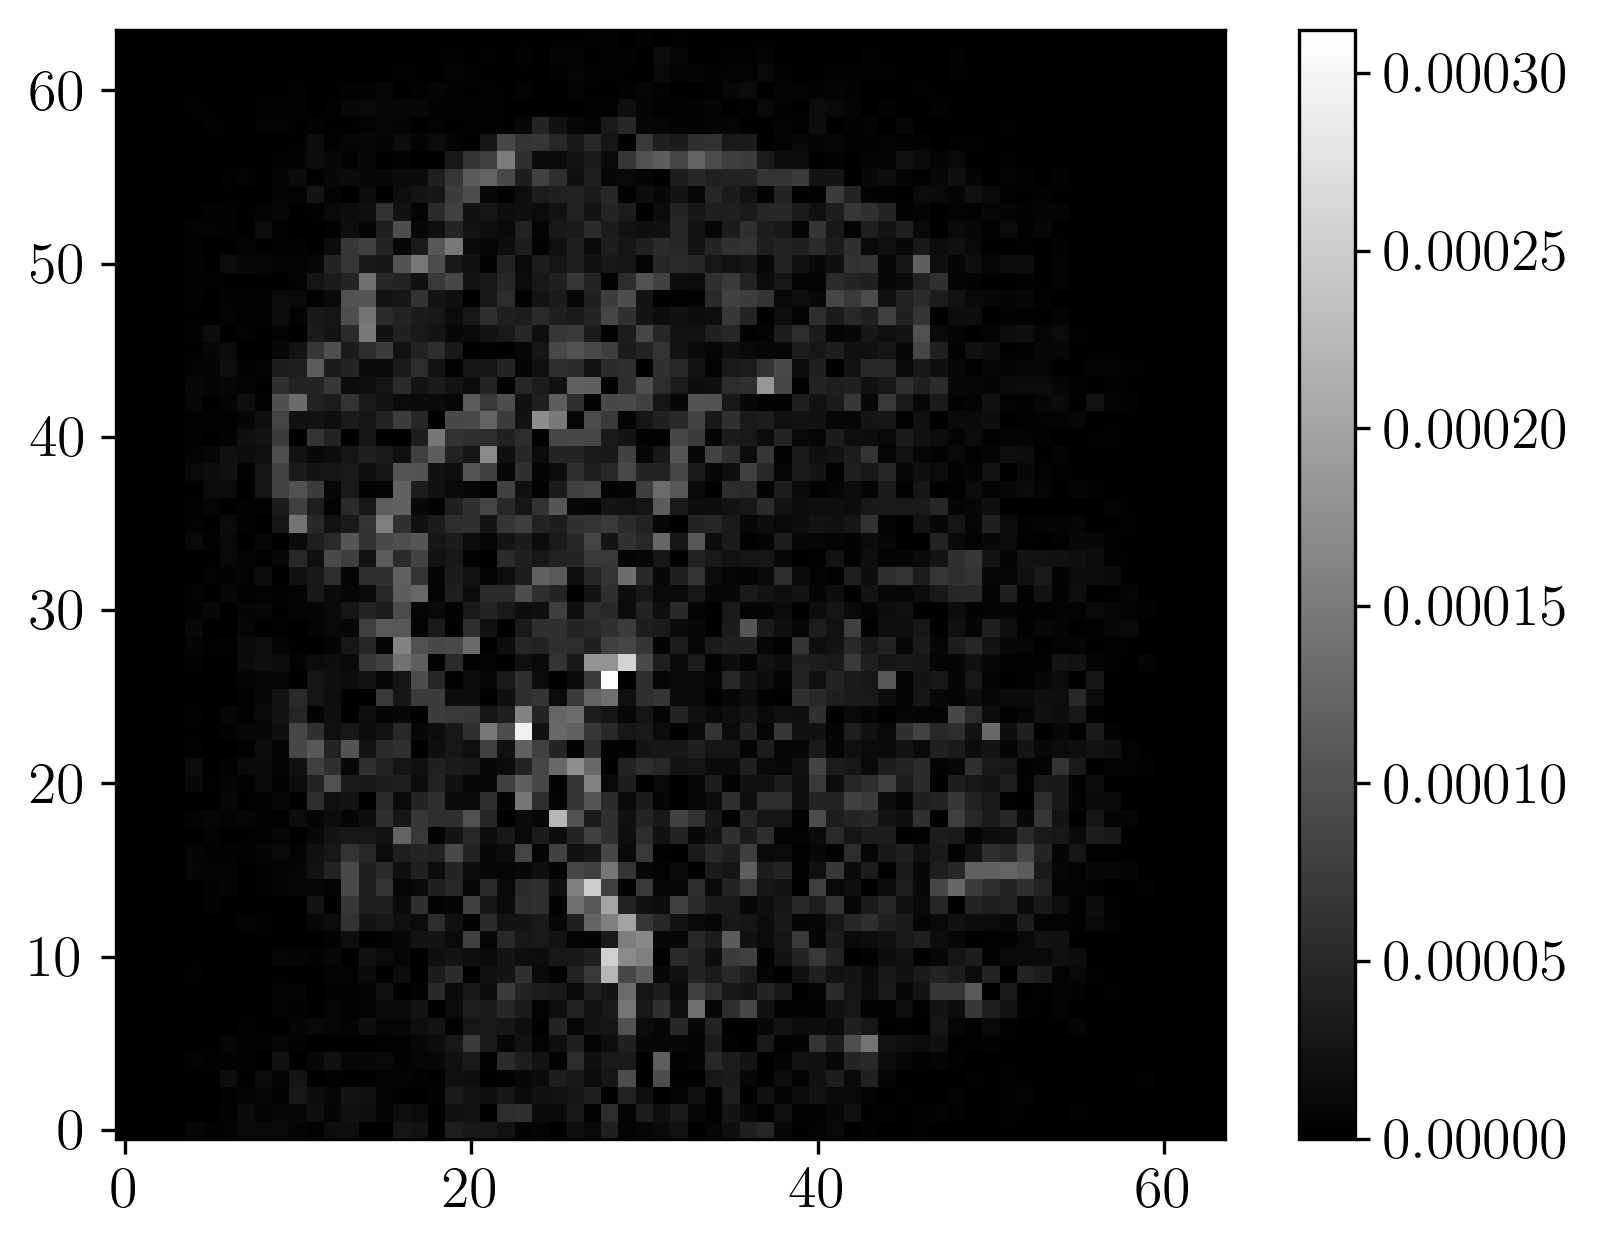
\includegraphics[width=0.33\textwidth]{default/sub-07-5-1-1000-37-20-_-_-difference.png}}}
	\caption{Slices of fMRI images from the test sample}
	\label{fig:example}
\end{figure}

\subsection{Delay time analysis}

The dependence of recovery quality on delay time was investigated.
The 47th subject and 4x compression were chosen for the example.
The left graph in Figure~\ref{fig:mse-dt} shows the dependence of the MSE metric
on the delay time $\Delta t$.
The study confirms that the most active part of the brain is the most active part of the brain 
in this examination~--- the occipital lobe.
The other parts contribute noise to the considered dependence.
In the present work, the above-mentioned region is localized, 
as shown in Figure~\ref{fig:local}.
To localize the region, the lower third and the right two thirds of the volumetric
of the tomographic image.
The area highlighted in red is the area that contains the 3\% 
of the most variable voxels in the occipital lobe.
For this purpose, all voxels of the localized area were ordered by 
descending order of the total absolute change in values.
Then 3\% of voxels with the largest changes were selected.
The MSE metric was recalculated exactly on this part of the image.
The corresponding graph is shown on the right side of Figure~\ref{fig:mse-dt}.
There is a more distinct minimum at $\Delta t \approx 5$ seconds.

\begin{figure}[h!]
	\centering
	\subfloat[True]{\label{fig:local-a}{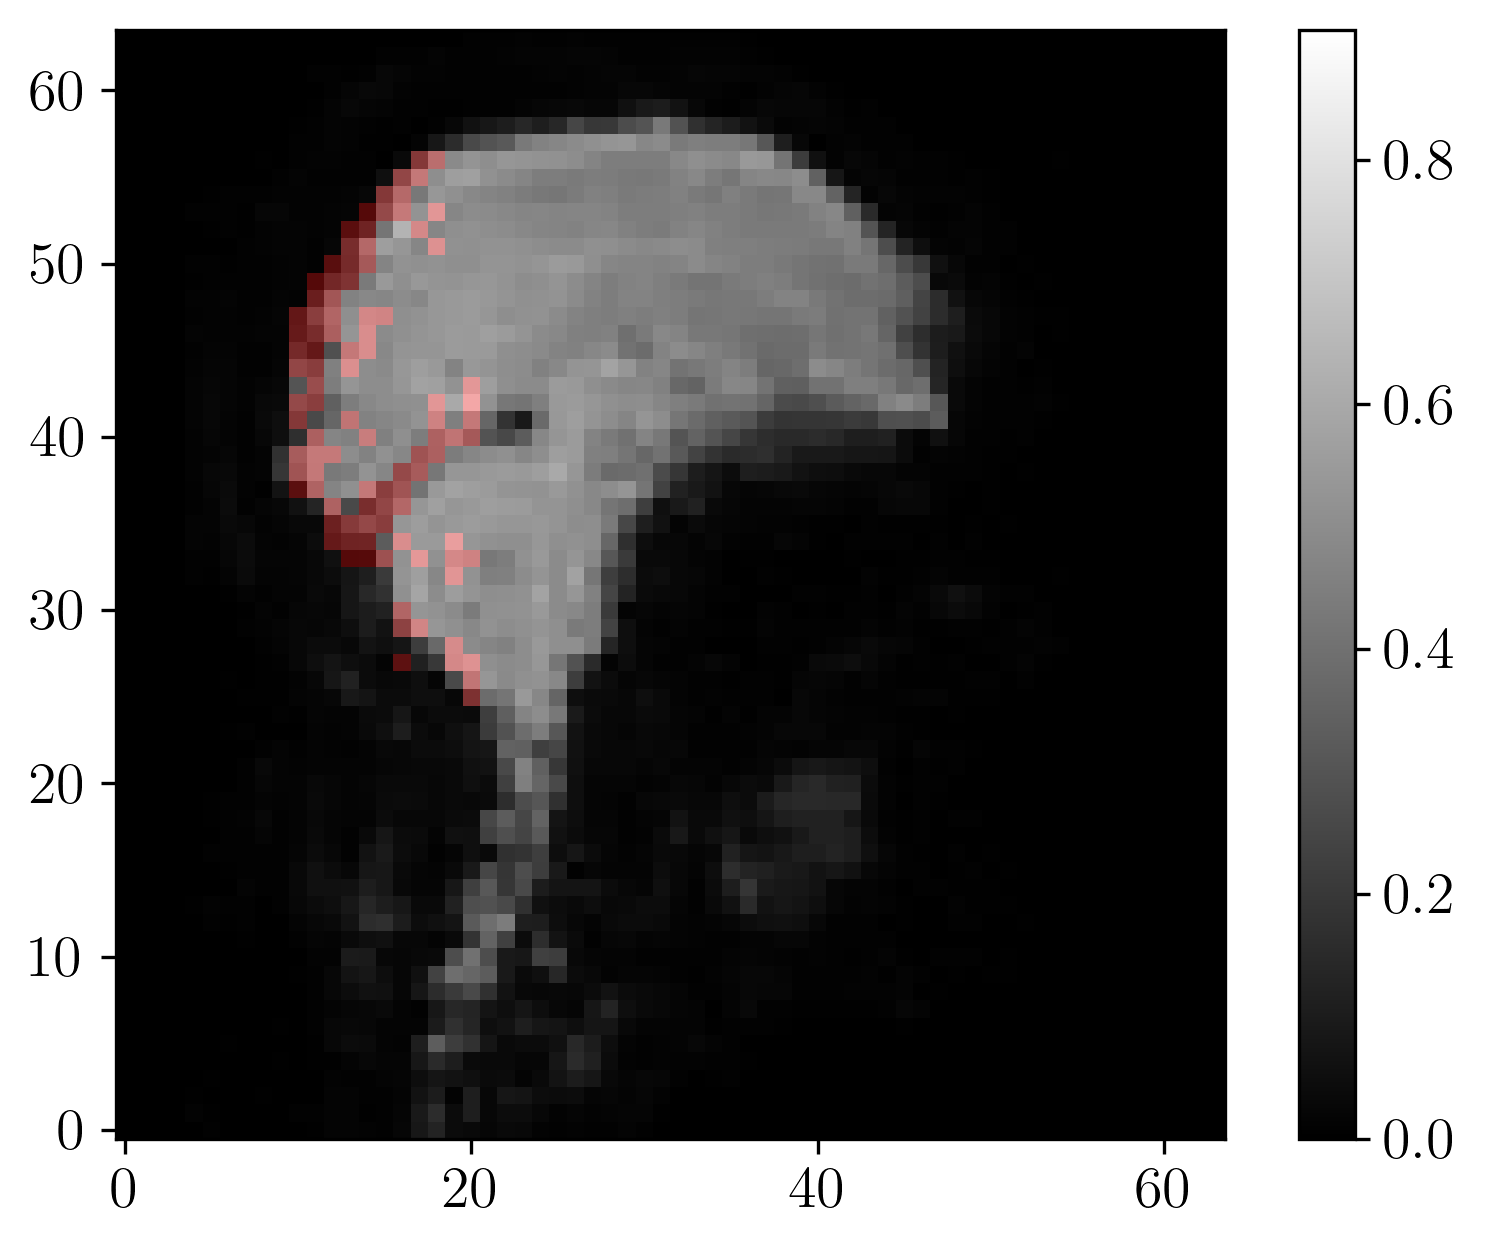
\includegraphics[width=0.33\textwidth]{local/sub-47-5-1-1000-37-20-_-_-test.png}}}
	\hfill
	\subfloat[Predicted]{\label{fig:local-b}{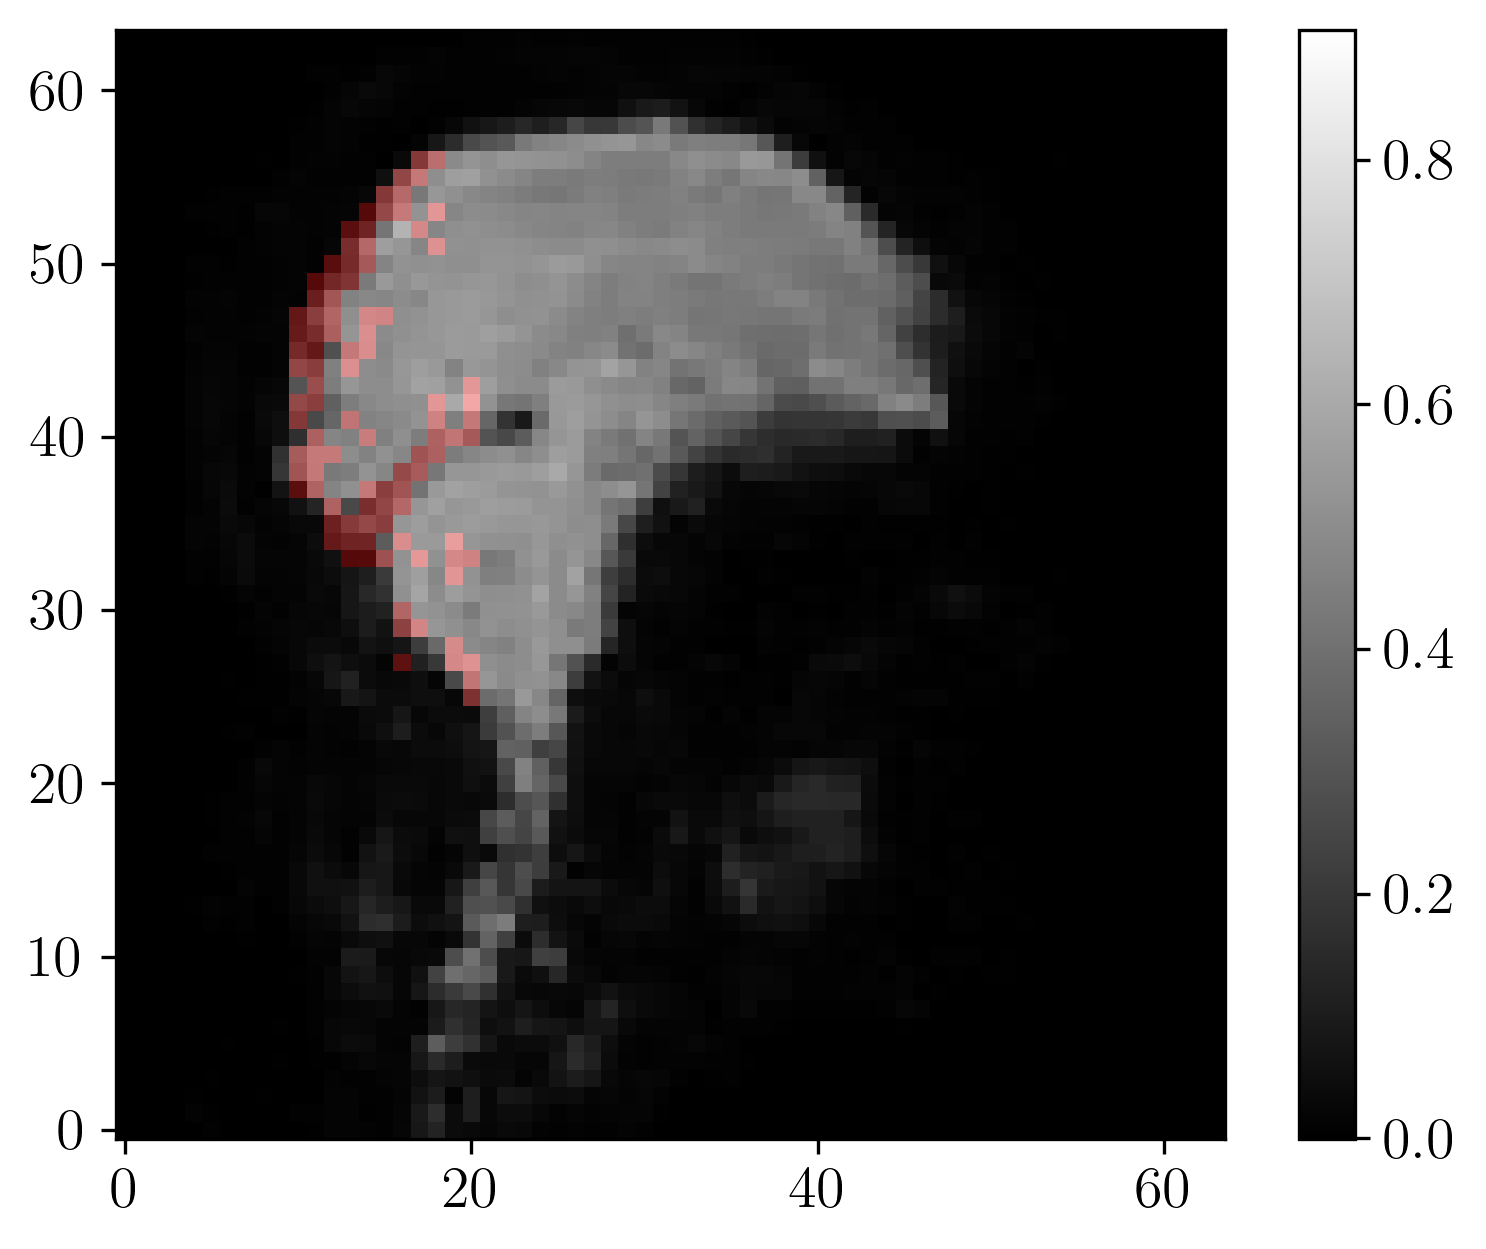
\includegraphics[width=0.33\textwidth]{local/sub-47-5-1-1000-37-20-_-_-predicted.png}}}
	\hfill
	\subfloat[Difference]{\label{fig:local-c}{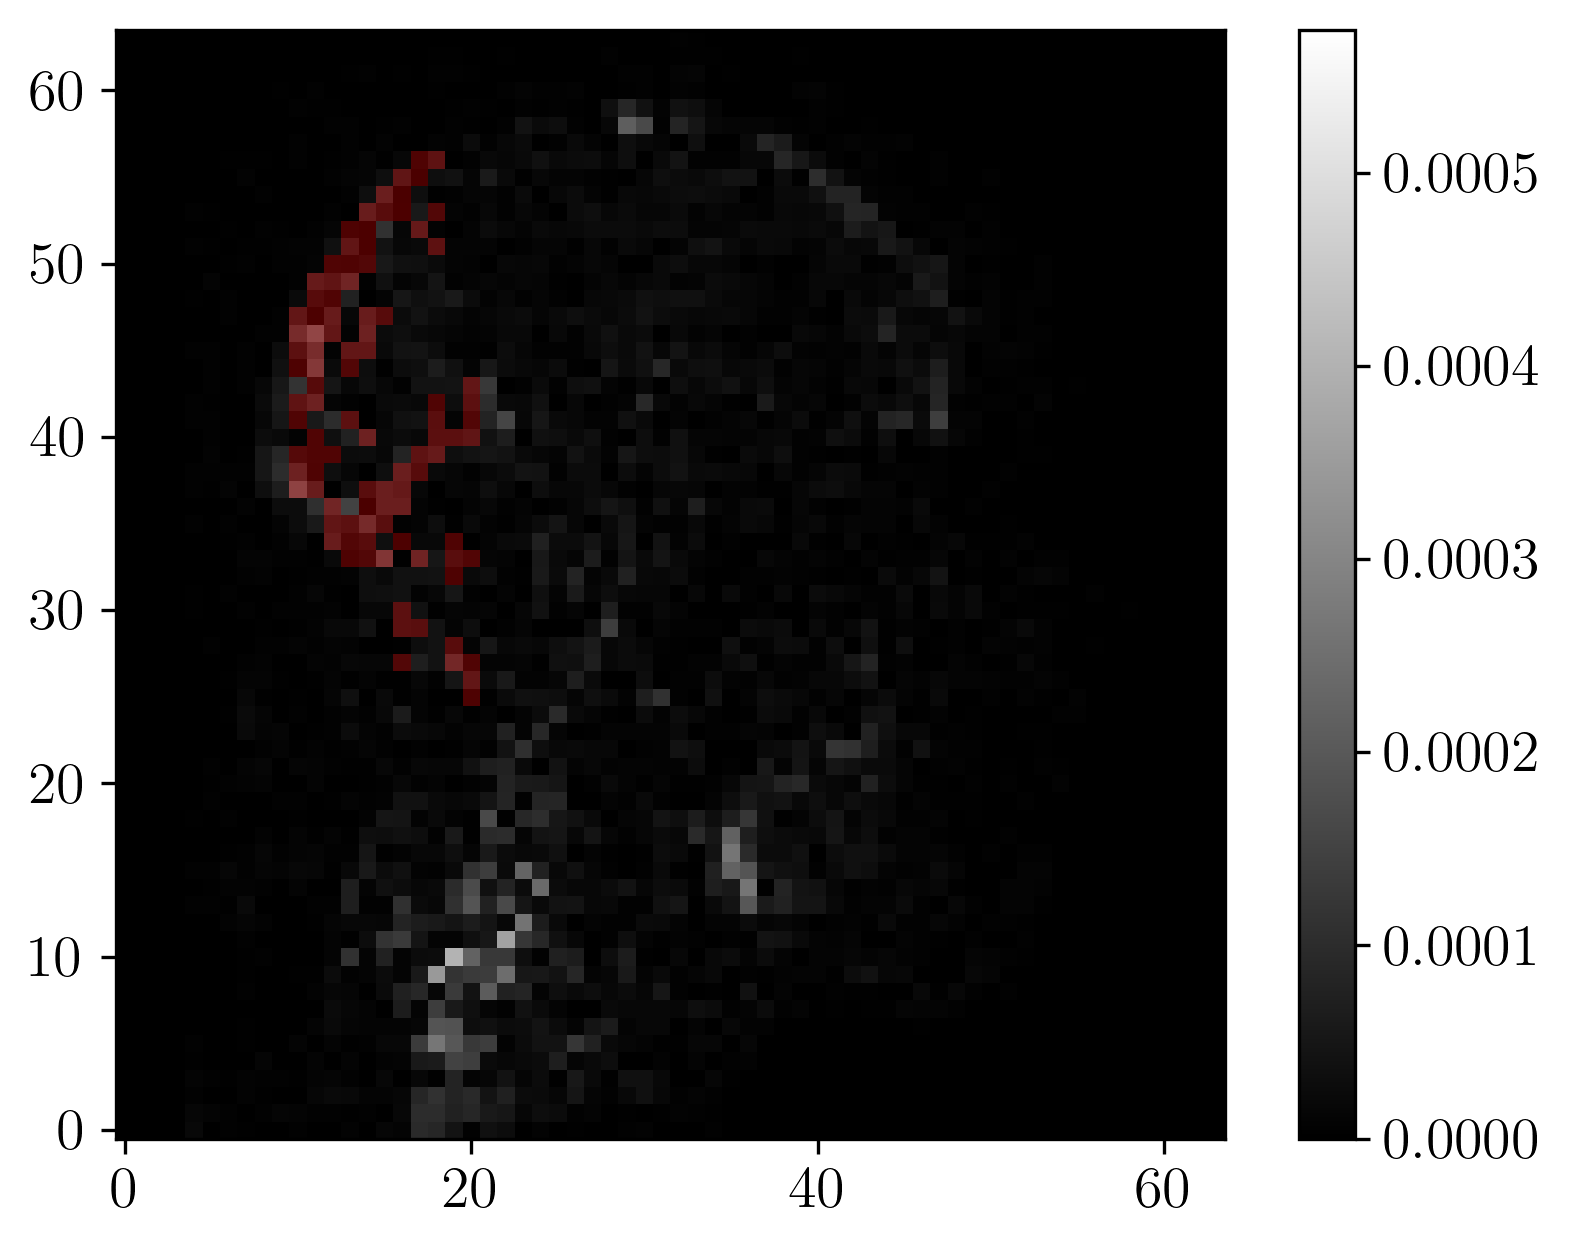
\includegraphics[width=0.33\textwidth]{local/sub-47-5-1-1000-37-20-_-_-difference.png}}}
	\caption{Localization of the most active zone}
	\label{fig:local}
\end{figure}

\begin{figure}[h!]
	\centering
	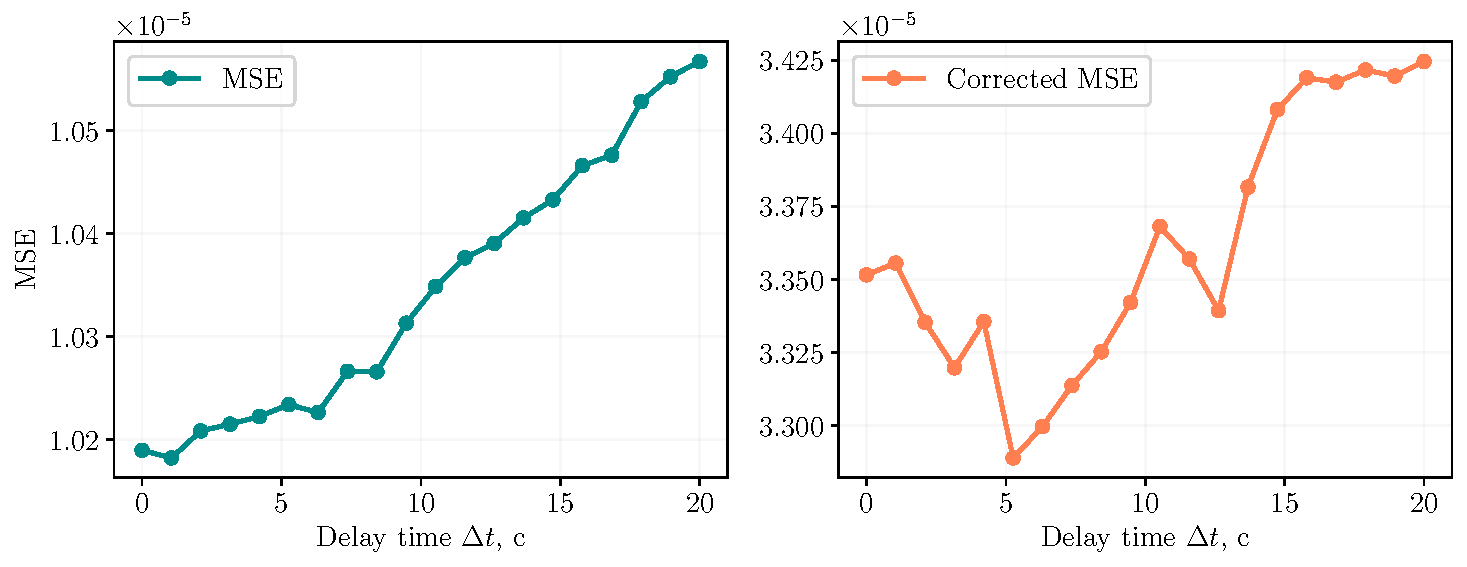
\includegraphics[width=\textwidth]{mse_dt.pdf}
	\caption{Dependence of MSE on delay time}
	\label{fig:mse-dt}
\end{figure}

\subsection{Optimal regularization parameter}

The dependence of MSE on the regularization parameter $\alpha$ was analyzed.
Compression factors 1, 2, 4, and 8 were considered.
The corresponding graphs are shown in Figure~\ref{fig:mse-alpha}.
Averaging over the subjects was performed to construct the graph.
The limits of standard deviation are marked.
The graphs show that the optimal value of the coefficient $\alpha \approx 1000$.
The curve shape is preserved regardless of the compression factor of fMRI images.

\begin{figure}[h!]
	\centering
	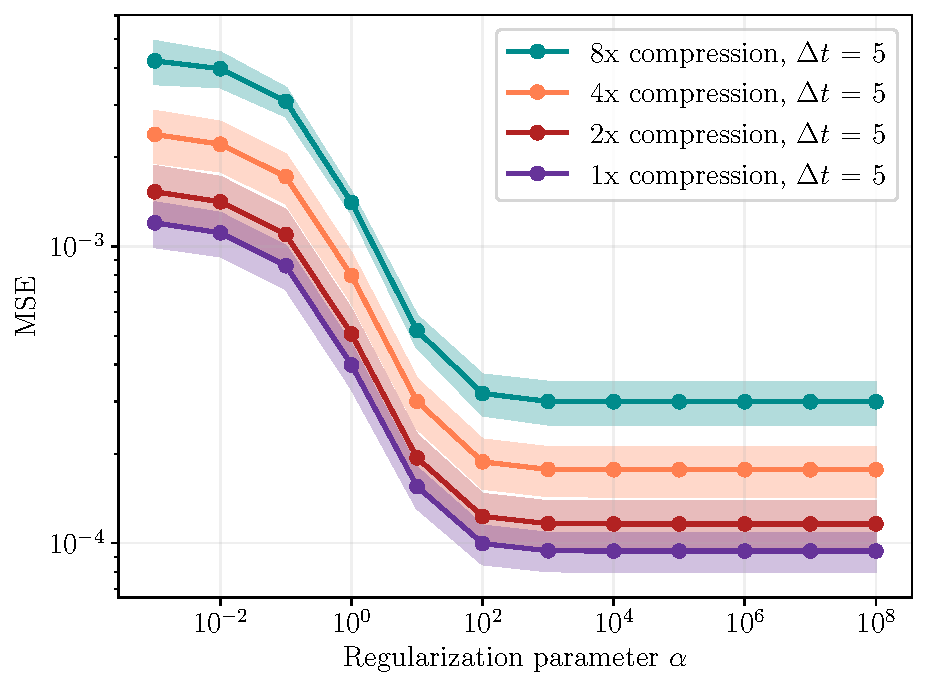
\includegraphics[width=0.65\textwidth]{subs_MSE_alpha.pdf}
	\caption{Dependence of MSE metric on regularization parameter $\alpha$ on images from the test sample}
	\label{fig:mse-alpha}
\end{figure}

\subsection{Effect of image compression ratio on method runtime}

We compare the training time of the model when using different
compression coefficients of fMRI images. Coefficients 1, 2, 4 and 8 are considered.
For each value of the compression ratio, the average value of the model training time for all subjects is calculated.
value of the model training time. The standard deviation is calculated.
The experimental results are summarized in Table~\ref{table:coeffs}.
The running time of the method is significantly reduced when using
pre-compression of fMRI images. 
The experiment with the selection of the optimal regularization coefficient
confirms that the compression of the images does not change the dependences.

\begin{table}[h!]
\caption{Dependence of model training time on compression ratio}\label{table:coeffs}
\begin{tabular}{@{}ccc@{}}
\toprule
Compression coefficient & Mean time, s & Std, s \\
\midrule
1 & 36.3 & 6.1 \\
2 & 6.7 & 0.5 \\
4 & 1.6 & 0.1 \\
8 & 1.4 & 0.3 \\
\botrule
\end{tabular}
\end{table}

\subsection{Analyzing the distribution of model weights}

A graph of the distribution of the values of the components of the model weight vector was plotted.
To construct it, we averaged over all voxels for the 4th subject.
The result is shown in Figure~\ref{fig:w-distr}.
The model weights do not lie in the neighborhood of any particular value, 
that is, their distribution is not degenerate.
This result is quite consistent with reality, because a human being, while viewing
pays attention to certain parts of the frame, such as characters or other details.
other details.

\begin{figure}[h!]
	\centering
	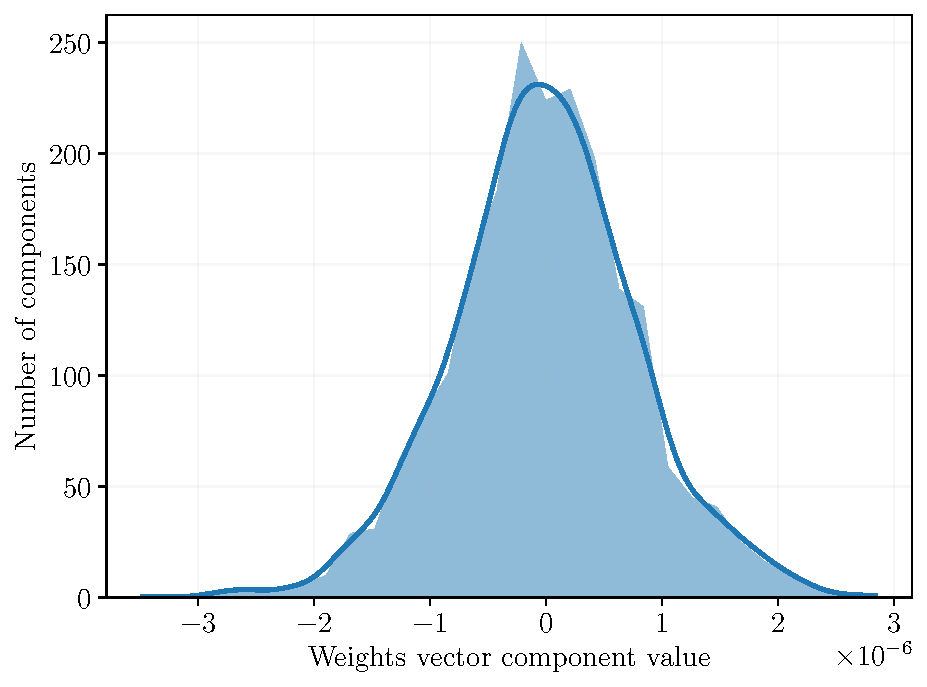
\includegraphics[width=0.65\textwidth]{distribution.pdf}
	\caption{Weights vector component distribution}
	\label{fig:w-distr}
\end{figure}

\subsection{Hypothesis of invariance of model weights with respect to humans}

The hypothesis of invariance of the model weights with respect to the person was tested:
Using one subject's weight matrix to reconstruct another subject's fMRI images.
The MSE metric on the test sample was used.
The results are presented in Table~\ref{table:inv}.
The 4th and 7th subjects were considered. The weight matrix of the 4th was used to reconstruct the
of the 7th subject's images.
The MSE values are almost the same.

\begin{table}[h!]
\caption{Testing the hypothesis of invariance of model weights with respect to humans}\label{table:inv}
\begin{tabular}{@{}cccc@{}}
\toprule
Weights matrix & True & Mixed  & Difference \\
\midrule
MSE & $6.3912 \cdot 10^{-5}$ & $6.3911 \cdot 10^{-5}$ & $1.37 \cdot 10^{-9}$ \\
\botrule
\end{tabular}
\end{table}

A similar experiment was conducted for each pair of subjects.
The obtained results are presented in Figure~\ref{fig:heatmap},
which was obtained as follows.
Some subject (corresponding to a row of the matrix) is considered, 
MSE~--- ``true" is calculated for him.
Next, another subject is considered (corresponding to a column of the matrix),
its matrix of weights is taken, and a prediction is made for the first subject, then the MSE~--- ``mixed" is calculated. 
The difference between the resulting MSE as a percentage of the ``true" is entered into the matrix.
A positive value means that the ``mixed" MSE is greater than the ``true".
A negative~--- that the ``mixed" is smaller.
That is, there is a MAPE on the heatmap.
The ideal model should result in only positive deviation values, however, as can be seen in Figure~\ref{fig:heatmap}, there are negative values in the matrix.
Nevertheless, they are rather small, namely, they correspond to deviations of the order of 1\%.
This is explained by the fact that the model is quite simple, and therefore has a
high generalizing ability.
However, this does not prevent us from concluding that the data do not contradict the hypothesis 
about the invariance of the model weights with respect to humans.

\begin{figure}[h!]
	\centering
	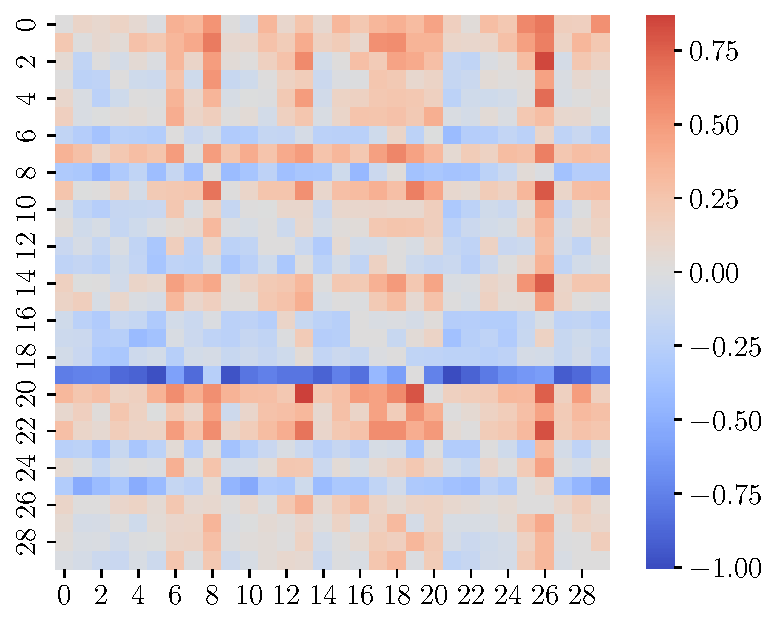
\includegraphics[width=0.5\textwidth]{heatmap.pdf}
	\caption{MAPE of MSE changing when predicting on the mixed weight matrix}
	\label{fig:heatmap}
\end{figure}

\subsection{Method corectness}

The quality of the method performance on uninformative data is considered.
A matrix consisting entirely of units was taken as a matrix of objects-signs $\mathbf{X}$.
Comparison with the results on the present feature-description matrix was made.
To the first snapshot of the 35th subject, all the reconstructed
changes in voxel values.
As a result, we have the last snapshot of the sequence. Figure~\ref{fig:recover}
are slices of the last true and recovered snapshots from the test sample.
Figure\myfigref{fig:recover}{fig:recover-c} shows the difference between them.
The results on the uninformative ones are demonstrated in Figure~\ref{fig:random}.
The difference between the true and recovered images when working with uninformative data
is much higher, which confirms that there is a correlation between the sensor readings and the
images from the video sequence. The numerical results are summarized in Table~\ref{table:random}.

\begin{figure}[h!]
	\centering
	\subfloat[True]{\label{fig:recover-a}{\includegraphics[width=0.33\textwidth]{original/sub-35-5-1-1000--1-20-_-_-recovered-test.png}}}
	\hfill
	\subfloat[Predicted]{\label{fig:recover-b}{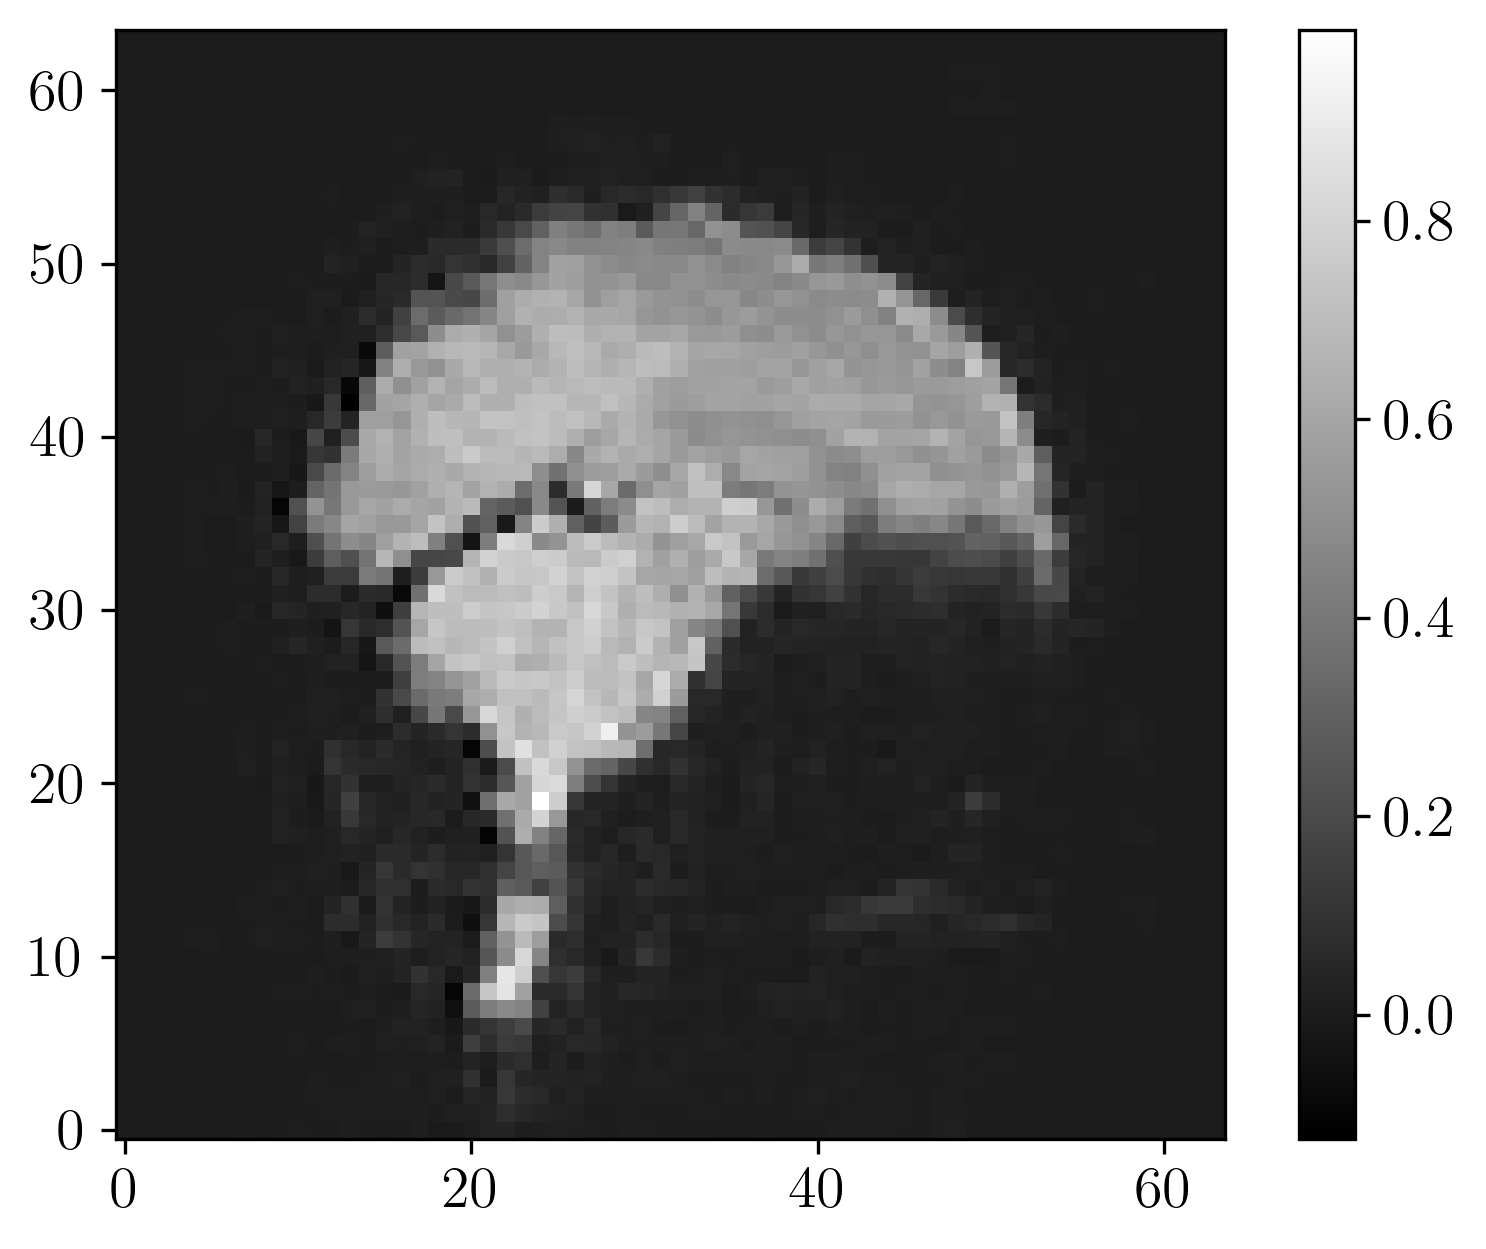
\includegraphics[width=0.33\textwidth]{original/sub-35-5-1-1000--1-20-_-_-recovered-predicted.png}}}
	\hfill
	\subfloat[Difference]{\label{fig:recover-c}{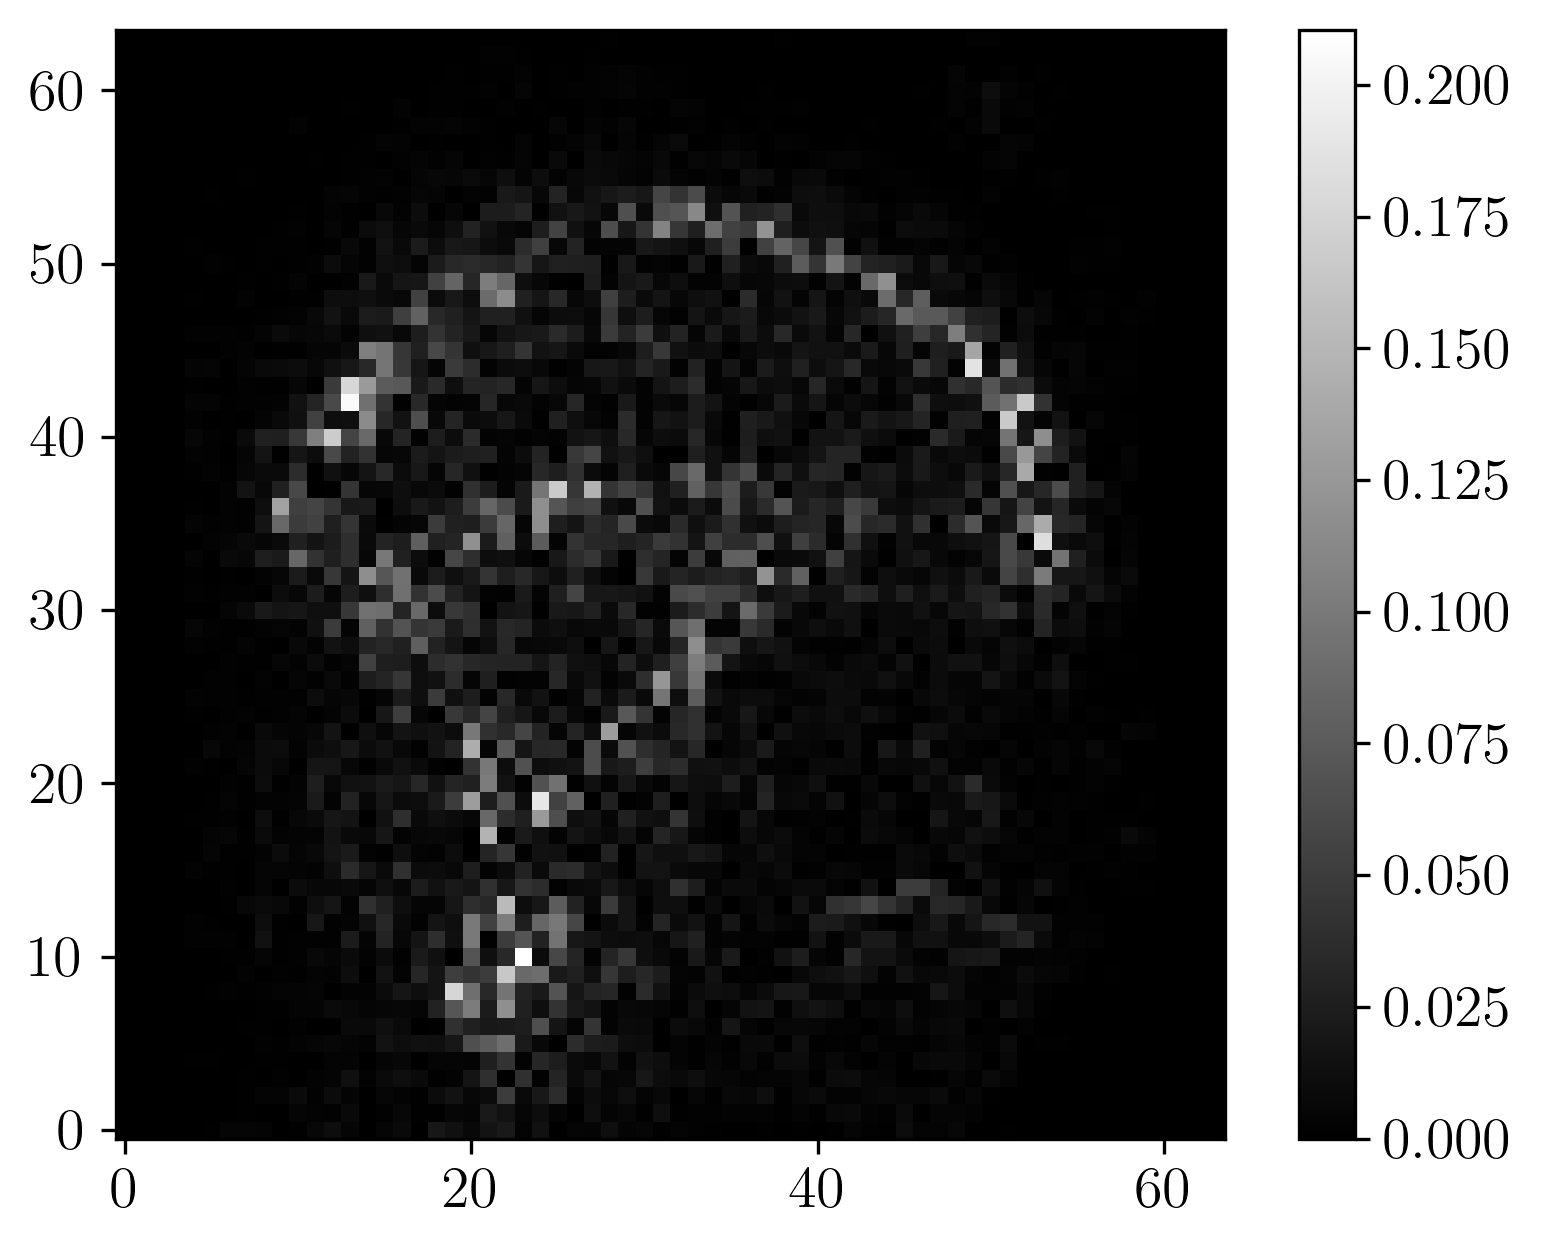
\includegraphics[width=0.33\textwidth]{original/sub-35-5-1-1000--1-20-_-_-recovered-difference.png}}}
	\caption{Slices of fMRI images from the test sample}
	\label{fig:recover}
\end{figure}

\begin{figure}[h!]
	\centering
	\subfloat[True]{\label{fig:random-a}{\includegraphics[width=0.33\textwidth]{noised/sub-35-5-1-1000--1-20-_-_-recovered-test.png}}}
	\hfill
	\subfloat[Predicted]{\label{fig:random-b}{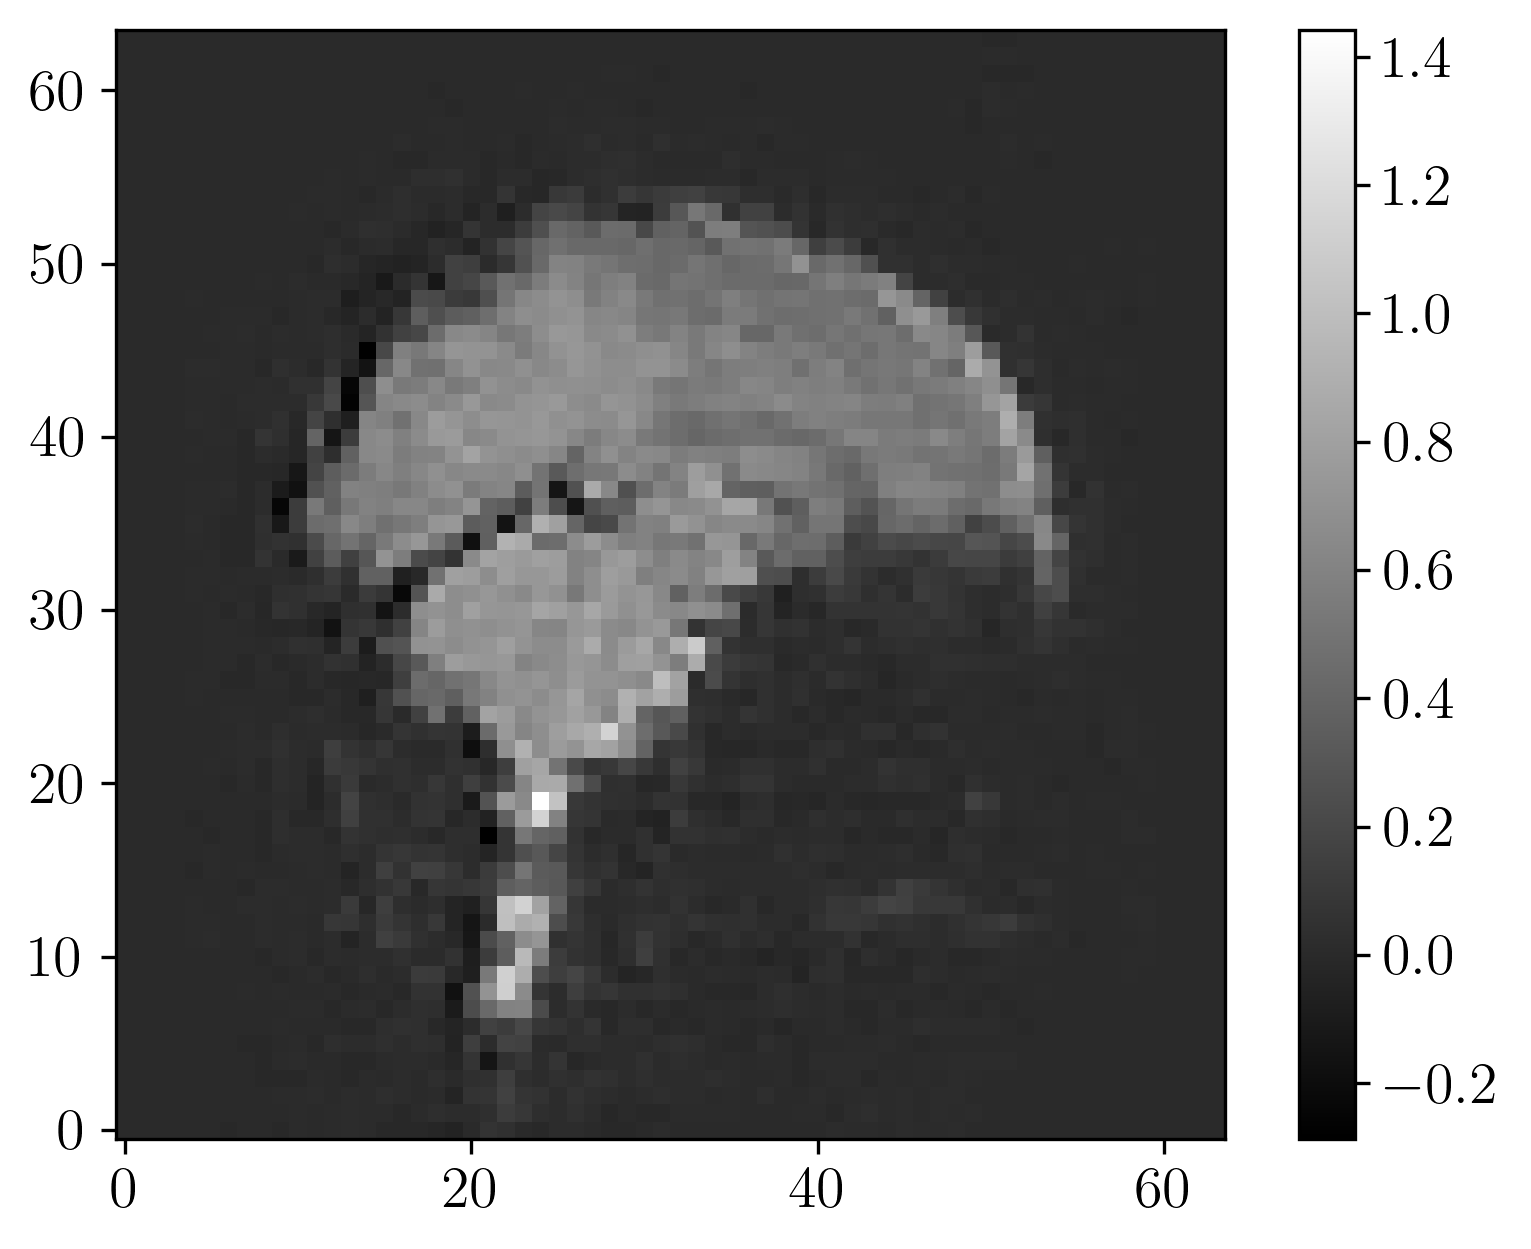
\includegraphics[width=0.33\textwidth]{noised/sub-35-5-1-1000--1-20-_-_-recovered-predicted.png}}}
	\hfill
	\subfloat[Difference]{\label{fig:random-c}{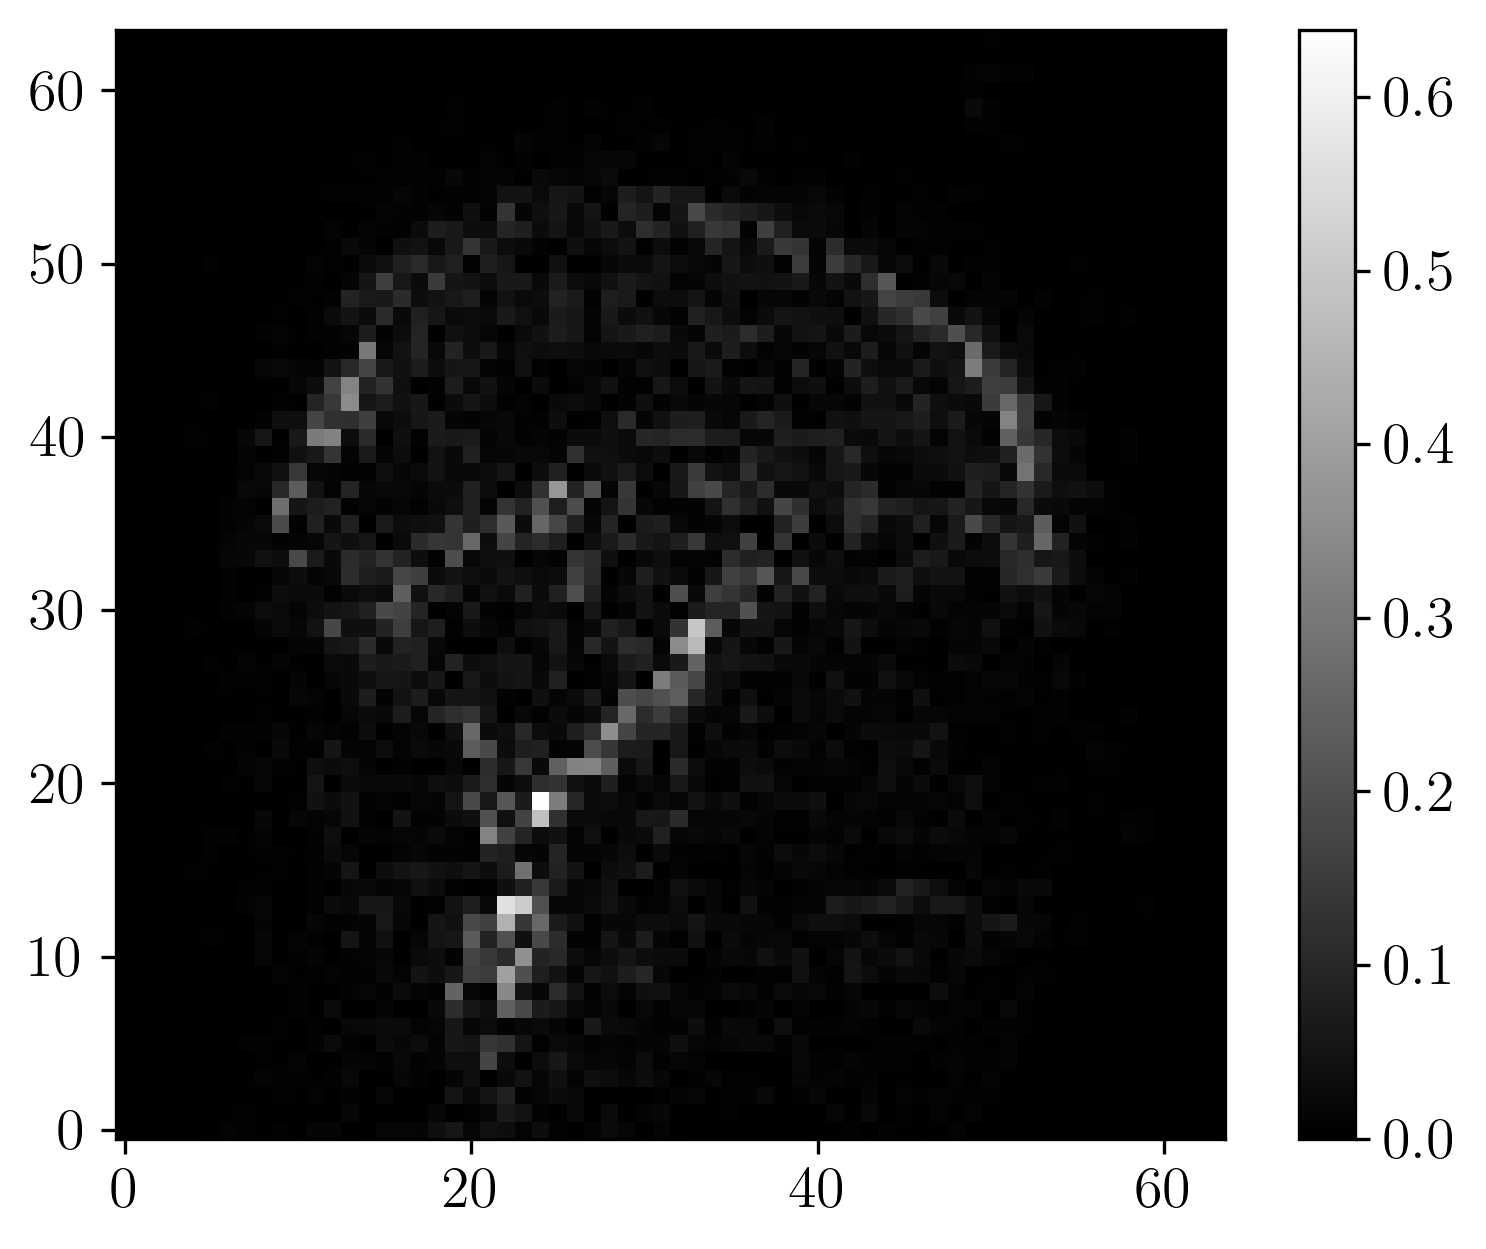
\includegraphics[width=0.33\textwidth]{noised/sub-35-5-1-1000--1-20-_-_-recovered-difference.png}}}
	\caption{Slices of fMRI images from the test sample (uninformative data)}
	\label{fig:random}
\end{figure}

\begin{table}[h!]
\caption{Quality of method performance on uninformative data}\label{table:random}
\begin{tabular}{@{}cccc@{}}
\toprule
Data & True & Uninformative & Difference \\
\midrule
MSE     & $3.67 \cdot 10^{-4}$ & $1.39 \cdot 10^{-3}$ & $1.02 \cdot 10^{-3}$ \\
\botrule
\end{tabular}
\end{table}

\section{Conclusion}

In this paper we consider the task of restoring the dependence between the readings fMRI sensors and human perception of the external world.
The method of approximation of fMRI images sequence by video sequence is proposed. 
The method takes into account the hemodynamic response time~--- the delay time between the images from the video sequence and the fMRI images. 
A linear model is independently constructed for each voxel of the fMRI image. 
Each linear model is constructed under the assumption that the sequence of fMRI images is Markovian. 
In the experiments, the optimal value of the delay time is selected for each subject. 
The optimal value is found from analyzing the plot of MSE versus delay time.
The regularization coefficient is selected. 
The effect of fMRI image compression ratio on model training time is investigated.
It is assumed that the occipital lobe of the brain is responsible for information from visual organs.
MSE correction is performed based on localization of this region and selection of the most changing voxels. 
With this construction, the graph has a characteristic minimum corresponding to the optimal value of the delay time.
The obtained value of the delay time is consistent with neurobiological information.
The experimental MSE values are small, indicating that there is a correlation between the data. 
The variation of images in the video sequence is taken into account since the distribution of model weights is not degenerate.
The hypothesis of invariance of model weights with respect to humans is tested. 
The correctness of the method is confirmed by experiments with random data.


\bibliography{references}% common bib file
%% if required, the content of .bbl file can be included here once bbl is generated
%%\input sn-article.bbl


\end{document}
